\documentclass[12pt,a4paper]{article}
\usepackage{amsmath}
\usepackage{amsfonts}
\usepackage{amssymb}
\usepackage{relsize}
\usepackage{tikz}
\usetikzlibrary{decorations.markings}
\usepackage[all]{xy}
\usepackage{listings}
\usepackage{enumerate}
\usepackage[a4paper,margin=1.3in,footskip=.5cm]{geometry}

%\includeonly{sections/observable}

\DeclareMathOperator{\im}{im}
\DeclareMathOperator{\id}{id}
\DeclareMathOperator{\rank}{rank}
\DeclareMathOperator{\card}{card}
\DeclareMathOperator{\coker}{coker}
\DeclareMathOperator{\colim}{colim}
\DeclareMathOperator{\rad}{rad}
\DeclareMathOperator{\Rect}{Rect}
\DeclareMathOperator{\Hom}{Hom}
\DeclareMathOperator{\Ob}{Ob}
\DeclareMathOperator{\End}{End}
\newcommand{\del}{\partial}

\newcommand{\R}{\mathbf{R}}
\renewcommand{\k}{\mathbf{k}}
\newcommand{\N}{\mathbf{N}}
\renewcommand{\S}{\mathbf{S}}
\newcommand{\T}{\mathbf{T}}
\newcommand{\W}{\mathbb{W}}
\newcommand{\U}{\mathbb{U}}
\newcommand{\V}{\mathbb{V}}
\newcommand{\I}{\mathbb{I}}
\newcommand{\J}{\mathbb{J}}
\newcommand{\A}{\mathsf{A}}
\newcommand{\B}{\mathsf{B}}
\newcommand{\M}{\mathsf{M}}
\renewcommand{\H}{\mathcal{H}}
\newcommand{\Dgm}{\mathsf{Dgm}}
\newcommand{\dgm}{\mathsf{dgm}}
\newcommand{\st}{\, \mid \,}
\newcommand{\C}{\mathcal{C}}
\newcommand{\D}{\mathcal{D}}
\newcommand{\natto}{\Rightarrow}

\newcommand{\rint}{\mathsmaller{\mathsmaller{\mathsmaller{\blacksquare}}}}

\usepackage{amsthm}
\newtheorem{theorem}{Theorem}[section]
\newtheorem{corollary}[theorem]{Corollary}
\newtheorem{lemma}[theorem]{Lemma}
\newtheorem{proposition}[theorem]{Proposition}
\theoremstyle{definition}
\newtheorem{example}[theorem]{Example}
\newtheorem{definition}[theorem]{Definition}
\makeatletter
\@addtoreset{theorem}{section}
\makeatother

%------------------------------------------------------------------------------------------
% quiver calculus commands
%------------------------------------------------------------------------------------------

\newcommand{\qlen}{1em}
\newcommand{\Qlen}{1.5em}
\newcommand{\QQlen}{3em}

\newcommand{\qem}{\makebox[\qlen]{---}}

% short
\newcommand{\qno}{\makebox[\qlen]{---}}  
\newcommand{\qon}[1]{\makebox[\qlen]{$_{\phantom{}}\bullet_{#1}$}}
\newcommand{\qoff}[1]{\makebox[\qlen]{$_{\phantom{}}\circ_{#1}$}}

% medium
\newcommand{\Qno}{\makebox[\Qlen]{--{}--{}--}}
\newcommand{\Qon}[1]{\makebox[\Qlen]{$_{\phantom{}}\bullet_{#1}$}}
\newcommand{\Qoff}[1]{\makebox[\Qlen]{$_{\phantom{}}\circ_{#1}$}}

% long
\newcommand{\QQno}{\makebox[\QQlen]{--{}--{}--{}--{}--{}--}}
\newcommand{\QQon}[1]{\makebox[\QQlen]{$_{\phantom{}}\bullet_{#1}$}}
\newcommand{\QQoff}[1]{\makebox[\QQlen]{$_{\phantom{}}\circ_{#1}$}}

\usepackage[backend=bibtex]{biblatex}
\addbibresource{persistenthomology.bib}

\begin{document}
\pagenumbering{gobble}

\newcommand{\HRule}{\rule{\linewidth}{0.5mm}}
\begin{titlepage}
\begin{center}
\textsc{\LARGE University of Queensland}\\[0.5cm]
\textsc{\Large Honours thesis}\\[1.5cm]

% Title
\HRule \\[0.4cm]
{ \huge \bfseries Persistence Modules over $\mathbf{R}$ \\[0.4cm] }

\HRule \\[1.5cm]

% Author and supervisor
\noindent
\begin{minipage}{0.4\textwidth}
\begin{flushleft} \large
\emph{Author:}\\
Mitchell Riley
\end{flushleft}
\end{minipage}%
\begin{minipage}{0.4\textwidth}
\begin{flushright} \large
\emph{Supervisor:} \\
A/Prof Benjamin Burton
\end{flushright}
\end{minipage}

\vfill

% Bottom of the page
{\large November 11, 2014}

\end{center}
\end{titlepage}

\clearpage
\vspace*{\fill}
%\thispagestyle{empty} 
\begin{quotation}
\emph{Persistence is to the character of man as carbon is to steel.}

\medskip
\raggedleft
\MakeUppercase{Napoleon Hill}

\end{quotation}
\vspace*{\fill}
\vspace*{\fill}
\newpage

\null\vspace{\fill} 
\renewcommand{\abstractname}{Acknowledgements}
\begin{abstract}
I would like to express my gratitude to my supervisor Ben Burton for putting up with my frequent changes in thesis topic and direction. I apologise that this computational topology project turned out to have little to do with computation or topology!

I also owe a debt to my fellow honours students, without whom this year would not have been nearly as much fun.	
\end{abstract}
\vspace{\fill}

\newpage
\tableofcontents
\newpage

\pagenumbering{arabic}
\setcounter{page}{1}
\section{Introduction}

Topological data analysis is an emerging field of applied algebraic topology that provides noise-resistant methods of interpreting real-world data. The cornerstone of topological data analysis is \emph{persistent homology}, a technique introduced by Zomorodian and Carlsson \cite{zomorodian2005computing} which relates topological features of a data set over different levels of detail. Each feature can be assigned an interval that describes the levels of detail at which it appears. The main insight is that any important feature of the data set will appear over a large interval. 

The algebraic object underlying persistent homology is the \emph{persistence module}, which is a diagram of vector spaces indexed by a partially ordered set. In practice, this indexing set is a finite subset of the natural numbers. Section~\ref{section-standard} shows that persistence modules of this sort have a simple structure, and always decompose into a sum of interval modules. Each interval is interpreted as a topological feature. 

This set of intervals is known as the \emph{persistence diagram} associated with the persistence module. One of the most important results on persistence diagrams is the stability theorem, which states that small changes in the initial data lead to small changes in the persistence diagram. This fact justifies the persistence diagram's use as an invariant of real-world data.

In proving this theorem, we need to pass to persistence modules indexed over the real line. Here we face a problem: not every persistence module decomposes as a sum of interval modules. Sections~\ref{section-modules} and \ref{section-diagrams} of this thesis are dedicated to working around this issue and finding an appropriate definition for persistence diagrams in this setting. Here we follow arguments made by Chazal et al. \cite{chazal2012structure}. With this foundation in place, we then prove the stability theorem in Section~\ref{section-stability}.

Finally, Sections~\ref{section-category-theory} and \ref{section-observable} follow a recent paper by Chazal, Crawley-Boevey and de Silva \cite{chazal2014observable} to show that, in a very precise sense, the difficulties we face above are all localised to the behaviour of persistence modules over infinitesimally small intervals. We define the category of persistence modules and relate it to the much better behaved `observable' category. This allows us to prove a strong structure theorem for persistence modules over the real numbers.

The main contribution of this thesis is a self-contained treatment of persistence modules over the real line, collecting results from many different sources. A number of proofs have been expanded or simplified from those that appear in the literature.
\section{Background Material}

We begin with a review of the material necessary to understand standard persistent homology. We use $\mathbf{N}$, $\mathbf{Z}$ and $\mathbf{R}$ to denote the natural numbers, integers and real numbers respectively, as we reserve blackboard bold to later denote persistence modules.

\subsection{Free modules}

\begin{definition}
A \emph{module over a ring $R$}, or \emph{$R$-module}, is an abelian group $M$ equipped with an action of $R$ satisfying the following properties. Let $1_R$ denote the multiplicative identity of the ring, and $rx$ the action of the ring element $r$ on the module element $x$. For any $r, s \in R$ and $x, y \in M$:
\begin{itemize}
\itemsep0em
\item $r(x + y) = rx + ry$;
\item $(r + s)x = rx + sx$;
\item $(rs)x = r(sx)$;
\item $1_R x = x$.
\end{itemize}
\end{definition}

\begin{example}
If we take $R$ to be a field, the above conditions are the conditions of a vector space, thus, a vector space over $F$ is precisely an $F$-module.
\end{example}

\begin{example}
Any abelian group $M$ is a $\mathbf{Z}$-module via the action $nx = \underbrace{x + \dots + x}_{n \text{ times}}$. Abelian groups are often referred to as $\mathbf{Z}$-modules for this reason.
\end{example}

\begin{definition}
The \emph{free $R$-module on a set $S$} is the module formed by taking every formal linear combination of elements of $S$ with coefficients in $R$. These linear combinations are given an $R$-module structure as follows. Let $a_i, b_i \in R$ and $s_i \in S$, then:
\begin{align*}
(a_1 s_1 + a_2 s_2 + \dots) + (b_1 s_1 + b_2 s_2 + \dots) &= (a_1 + b_1) s_1 + (a_2 + b_2) s_2 + \dots; \\
a (a_1 s_1 + a_2 s_2 + \dots) &= (a a_1) s_1 + (a a_2) s_2 + \dots
\end{align*}

The \emph{free abelian group on $S$} is the free $\mathbf{Z}$-module on $S$.
\end{definition}

\subsection{Graded rings and modules}

\begin{definition}
A \emph{graded ring} is a ring with a decomposition into abelian groups:
\begin{align*}
  R = \bigoplus_{n \in \mathbf{N}} R_n
\end{align*}
such that multiplication satisfies $R_n R_m \subseteq R_{n+m}$. Elements of any $R_n$ are called \emph{homogeneous elements of degree $n$} and for any $r \in R_n$ we write $\deg r = n$.
\end{definition}

\begin{example}
The prototypical example of a graded ring is the polynomial ring $R[t]$, which decomposes as:
\begin{align*}
  R[t] = \bigoplus_{n \in \mathbf{N}} t^n \cdot R.
\end{align*}
\end{example}

Given a module over a graded ring, we can have the module structure respect the grading of the ring.

\begin{definition}
A \emph{graded module} over a graded ring $R$ is a module $M$ with a decomposition:
\begin{align*}
  M = \bigoplus_{n \in \mathbf{N}} M_n
\end{align*}
where the action of $R$ satisfies $R_n M_m \subseteq M_{n+m}$.
\end{definition}

We will see that the structure of standard persistent homology is equivalent to a graded module over a particular ring.

\subsection{Structure theorem}

Recall that a \emph{principal ideal domain} (PID) is an integral domain in which every ideal is generated by one element. Such ideals are called \emph{principal} ideals.

\begin{example}
The integers $\mathbf{Z}$ are a simple example of a PID. Given any ideal, we can find the greatest common divisor of all its elements. This element must generate the whole ideal.

For an example of a ring that is \emph{not} a PID, consider the ring $\mathbf{Z}[x]$. The ideal $\langle x, 2 \rangle$ cannot be generated by one element.
\end{example}

\begin{example}
For our purposes, an important example of a PID is the polynomial ring $\k[x]$, where $\k$ is a field.
\end{example}

Finitely generated modules over a PID can be uniquely decomposed using a generalisation of the structure theorem for finitely generated abelian groups \cite{dummit-foote}.

\begin{theorem}
If $R$ is a PID, every finitely generated module over $R$ is isomorphic to one of the form
\begin{align*}
R^\beta \oplus \left( \bigoplus_{i=1}^m R / \langle d_i \rangle \right)
\end{align*}
where $d_i \in R$, $\beta \in \mathbf{N}$, and $d_i \mid d_{i+1}$.
\end{theorem}

When $R = \mathbf{Z}$, we recover the structure theorem for finitely generated abelian groups. Given a graded module, we can say more:

\begin{theorem}
\label{thm:graded-pid-structure}
Every graded module over a PID $R$ is isomorphic to one of the form
\begin{align*}
\left( \bigoplus_{i=1}^n \Sigma^{\alpha_i} R \right) \oplus \left( \bigoplus_{i=1}^m \Sigma^{\gamma_i} R / \langle d_i \rangle \right)
\end{align*}
where $d_i \in R$ are homogeneous elements with $d_i | d_{i+1}$, $\alpha_i, \gamma_j \in \N$. The symbol $\Sigma^k$ denotes a formal upward shift of $k$ steps in the grading, i.e., $\Sigma^k R$ is the graded ring with $(\Sigma^k R)_n = R_{n - k}$.
\end{theorem}

\subsection{Simplicial complexes}
To begin with, we restrict our focus to a class of topological spaces that have a particularly simple description: simplicial complexes. Intuitively, these are spaces constructed of vertices, edges, triangles, tetrahedra, and so on, with these shapes glued together along their `faces'.

\begin{definition}
An \emph{abstract simplicial complex} $K = (V, S)$ is a set $V$ together with a collection $S$ of subsets of $V$ called \emph{simplices} such that for every $v \in V$, $\{v\} \in S$, and if $\tau \subseteq \sigma \in S$, then also $\tau \in S$.

The subsets $\{v\}$ of $V$ are called the \emph{vertices} of $K$. A simplex $\sigma \in S$ is of dimension $k$ if $\sigma$ has $k+1$ elements. If $\tau \subset \sigma$, we say $\tau$ is a \emph{face} of $\sigma$.

An \emph{oriented} simplex is a simplex together with a choice of orientation for that simplex. Any ordering of the vertices determines an orientation, and two orientations are considered equivalent if they differ by an even permutation. We write $[\omega]$ for an oriented simplex, and use the ordered sequence $[v_1, v_2, \dots]$ to denote the oriented simplex with vertices $\{v_1, v_2, \dots \}$ and the given orientation.
\end{definition}

\begin{example}
We will use the following simplicial complex as a running example. Let $K = (V, S)$ with:
\begin{align*}
  V &= \{a, b, c, d\} \\
  S &= \{\emptyset, \{a\}, \{b\}, \{c\}, \{d\}, \{a, b\}, \{a, c\}, \{a, d\}, \{b, d\}, \{d, c\}, \{a, b, d\}\}
\end{align*}
\end{example}

Abstract simplicial complexes are useful in practice because of their simple structure and combinatorial properties. In theoretical settings, it is more convenient to consider general topological spaces.

We can associate a topological space to an abstract simplicial complex by pairing each $k$-dimensional subset in $S$ with the convex hull of $k+1$ independent points in $\mathbf{R}^d$ for some $d \geq k$. Such a space is called a \emph{geometric realisation}. With this pairing we recover the notions of shape we are familiar with: 1-simplices correspond to edges, 2-simplices to triangles and so on. In such a realisation we require that the nontrivial intersection of any two simplices is one of their common faces.

\begin{figure}[h]
\centering
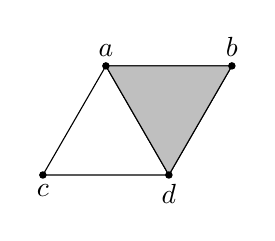
\begin{tikzpicture}[scale=0.4]
  \coordinate[label=above:$a$] (a) at (2,3.464);
  \coordinate[label=above:$b$] (b) at (6,3.464);
  \coordinate[label=below:$c$] (c) at (0,0);
  \coordinate[label=below:$d$] (d) at (4,0);

  \draw (a) -- (d) -- (c) -- cycle;
  \draw (d) -- (b) -- (a);
  \draw[fill=gray!50] (a) -- (d) -- (b) -- cycle;
  \draw[black,fill] (a) circle [radius=0.1cm] ;
  \draw[black,fill] (b) circle [radius=0.1cm] ;
  \draw[black,fill] (c) circle [radius=0.1cm] ;
  \draw[black,fill] (d) circle [radius=0.1cm] ;
\end{tikzpicture}
\caption{The simplicial complex $K$}
\label{fig:simplicial}
\end{figure}

\begin{example}
Figure~\ref{fig:simplicial} shows one realisation of our abstract simplicial complex $K$.
\end{example}

Given any abstract simplicial complex $K$, we can always construct a geometric realisation.

\begin{theorem}
Every abstract simplicial complex has a geometric realisation.
\end{theorem}
\begin{proof}
Let $n$ be the number of vertices in the simplicial complex $K$. Choose a one-to-one correspondence between the vertices of $K$ and the unit vectors $\{e_1, e_2, \dots, e_n\}$ in $\mathbf{R}^n$. For each simplex in $K$, construct the convex hull of the corresponding points in $\mathbf{R}^n$. By construction, these convex hulls intersect either on a common face or not at all. Our geometric realisation is the union of these convex hulls, inheriting the subspace topology of $\mathbf{R}^n$.
\end{proof}

We will refer to an abstract simplicial complex and its realisation interchangeably.

\subsection{Simplicial homology}

Homology is a procedure that, given a topological space, produces a sequence of abelian groups, $H_k$, that represent the `holes' in the space. This set of groups is a topological invariant; any two homeomorphic spaces have the same homology groups. There are a number of different types of homology. We begin by introducing simplicial homology, which can only be applied to simplicial complexes.

The $k$-th homology group, $H_k(K)$, describes the $k$-dimensional holes in $K$. For example, the `hole' in the middle of a circle is a 1-dimensional hole, so $H_1(\mathbb{S}^1)$ has rank 1. A 0-dimensional hole is interpreted as a gap between two components, so $H_0$ counts the path-connected components of $K$.

\begin{example}
Consider the $n$-sphere $\mathbb{S}^n$. The homology groups are as follows:
\begin{align*}
  H_k(\mathbb{S}^n) = \begin{cases}
    \mathbf{Z} & k = 0 \text{ or } n ;\\
    0 & \text{otherwise.}
\end{cases}
\end{align*}
The non-trivial $H_0$ represents the single connected component of $\mathbb{S}^n$, and non-trivial $H_n$ the $n$-dimensional hole.
\end{example}

\begin{example}
Consider the standard embedding of a torus $\mathbb{T}$ in $\R^3$. The torus has a single component, two 1-dimensional holes (one circle through the middle, one running around the loop), and one 2-dimensional hole (the void inside the torus). The corresponding homology groups are:
\begin{align*}
  H_k(\mathbb{T}) = \begin{cases}
    \mathbf{Z} & k = 0 \\
    \mathbf{Z} \oplus \mathbf{Z} & k = 1 \\
    \mathbf{Z} & k = 2 \\
    0 & \text{otherwise.}
\end{cases}
\end{align*}
\end{example}

\begin{definition}
The \emph{$k$-th chain group} of $K$, denoted $C_k$, is the free abelian group with basis the set of oriented simplices of $K$, where we let $[\sigma] = -[\tau]$ if $\sigma$ and $\tau$ are the same simplex with the opposite orientation.
\end{definition}

Elements of $C_k$ are known as $k$-chains, and have the form $c = \sum_i n_i [\sigma_i]$, with $\sigma_i$ $k$-simplices in $K$.

Let $\sigma$ be a $k$-simplex with vertices $[v_0, \cdots, v_k]$. Given such a $k$-simplex, we would like to calculate its boundary, $\del_k \sigma$. The faces of $\sigma$ are the $(k-1)$-simplices with vertex sets of the form $[v_0, \cdots, \hat{v_i}, \cdots, v_k]$, where $\hat{v_i}$ indicates that $v_i$ is deleted from the sequence. We might expect the boundary to be the chain given by the sum of the faces, but a better choice is the following
\begin{align*}
\del_k[\sigma] = \del_k[v_0, \cdots, v_k] = \sum_i (-1)^i [v_0, \cdots, \hat{v_i}, \cdots, v_k].
\end{align*}
When the dimension is unambiguous, we write $\del$ for $\del_k$.

\begin{example}
For generic simplices of dimension 0,1,2:
\begin{align*}
  &\del[v_0] = 0 \\
  &\del[v_0, v_1] = [v_1] - [v_0] \\
  &\del[v_0, v_1, v_2] = [v_1, v_2] - [v_0, v_2] + [v_0, v_1]
\end{align*}
\end{example}

Intuitively, we make this definition so that orientations are kept consistent as we travel around the boundary of a simplex.

The boundary operator $\del_k$ can be turned into a homomorphism $C_k \to C_{k-1}$ by extending it linearly on the basis elements of $C_k$. Together, these groups and maps form what is known as a \emph{chain complex}, $C_*$.
\begin{displaymath}
\xymatrix{
\cdots \ar[r] & C_{k+1} \ar[r]^{\del_{k+1}} & C_{k} \ar[r]^{\del_k} & C_{k-1} \ar[r] & \cdots
}
\end{displaymath}

The boundary operator allows us to define two important subgroups of each $C_k$: the \emph{cycle group} $Z_k = \ker \del_k$ and the \emph{boundary group} $B_k = \im \del_{k+1}$. These groups match with our intuition of what a cycle and boundary should be; a cycle generalises a closed loop or surface, and a boundary is a cycle that bounds a higher dimensional shape.

\begin{figure}[h]
\centering
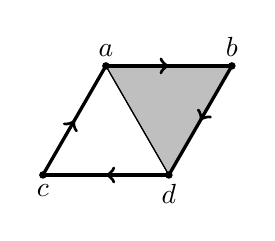
\begin{tikzpicture}[scale=0.4]
  \coordinate[label=above:$a$] (a) at (2,3.464);
  \coordinate[label=above:$b$] (b) at (6,3.464);
  \coordinate[label=below:$c$] (c) at (0,0);
  \coordinate[label=below:$d$] (d) at (4,0);

  \draw[fill=gray!50] (a) -- (d) -- (b) -- cycle;
  \begin{scope}[very thick,decoration={
      markings,
      mark=at position 0.5 with {\arrow{>}}}
      ]
      \draw[postaction={decorate}] (a) -- (b);
      \draw[postaction={decorate}] (b) -- (d);
      \draw[postaction={decorate}] (d) -- (c);
      \draw[postaction={decorate}] (c) -- (a);
  \end{scope}

  \draw (a) -- (d);
  \draw[black,fill] (a) circle [radius=0.1cm] ;
  \draw[black,fill] (b) circle [radius=0.1cm] ;
  \draw[black,fill] (c) circle [radius=0.1cm] ;
  \draw[black,fill] (d) circle [radius=0.1cm] ;
\end{tikzpicture}
\caption{$K$ with the cycle $[a, b] + [b, d] - [c, d] - [a, c]$ highlighted}
\label{fig:cycle}
\end{figure}

\begin{figure}[h]
\centering
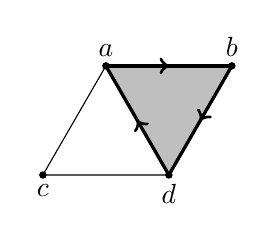
\begin{tikzpicture}[scale=0.4]
  \coordinate[label=above:$a$] (a) at (2,3.464);
  \coordinate[label=above:$b$] (b) at (6,3.464);
  \coordinate[label=below:$c$] (c) at (0,0);
  \coordinate[label=below:$d$] (d) at (4,0);

  \draw[fill=gray!50] (a) -- (d) -- (b) -- cycle;
  \begin{scope}[very thick,decoration={
      markings,
      mark=at position 0.5 with {\arrow{>}}}
      ]
      \draw[postaction={decorate}] (a) -- (b);
      \draw[postaction={decorate}] (b) -- (d);
      \draw[postaction={decorate}] (d) -- (a);
  \end{scope}

  \draw (a) -- (c) -- (d);
  \draw[black,fill] (a) circle [radius=0.1cm] ;
  \draw[black,fill] (b) circle [radius=0.1cm] ;
  \draw[black,fill] (c) circle [radius=0.1cm] ;
  \draw[black,fill] (d) circle [radius=0.1cm] ;
\end{tikzpicture}
\caption{$K$ with the boundary $\del [a, b, d]$ highlighted}
\label{fig:boundary}
\end{figure}

\begin{example}
Returning to our earlier example, the chain $[a, b] + [b, d] - [c, d] - [a, c]$ is an element of $Z_1$, as:
\begin{align*}
  \del([a, b] + [b, d] - [c, d] - [a, c]) &= \del[a, b] + \del[b, d] - \del[c, d] - \del[a, c] \\
  &= ([b] - [a]) + ([d] - [b]) - ([d] - [c]) - ([c] - [a]) \\
  &= 0
\end{align*}
We represent an oriented simplex $[x, y]$ as an arrow pointing $x \to y$. This chain is shown in Figure~\ref{fig:cycle}.

The chain $\del [a,b,d] = [b, d] - [a, d] + [a, b]$ is an element of $B_1$. This chain is shown in Figure~\ref{fig:boundary}. In fact, this chain is a generator for the group $B_1$, as $[a,b,d]$ is the only 2-simplex. Note the consistent orientation of the edges.
\end{example}

\begin{proposition}
For any $k$, $\del_{k-1} \circ \del_k = 0$.
\end{proposition}
\begin{proof}
By definition,
\begin{align*}
\del_k[v_0, \cdots, v_k] = \sum_i (-1)^i [v_0, \cdots, \hat{v_i}, \cdots, v_k]
\end{align*}
Then,
\begin{align*}
\del_{k-1}\del_k[v_0, \cdots, v_k] &= \sum_{j<i} (-1)^i (-1)^j [v_0, \cdots, \hat{v_j}, \cdots, \hat{v_i}, \cdots, v_k] \\
& \quad + \sum_{j>i} (-1)^i (-1)^{j-1} [v_0, \cdots, \hat{v_i}, \cdots, \hat{v_j}, \cdots, v_k] \\
&= \sum_{j<i} (-1)^i (-1)^j [v_0, \cdots, \hat{v_j}, \cdots, \hat{v_i}, \cdots, v_k] \\
& \quad - \sum_{j<i} (-1)^i (-1)^j [v_0, \cdots, \hat{v_j}, \cdots, \hat{v_i}, \cdots, v_k] \\
&= 0
\end{align*}
where in the second sum we swap the roles of $i$ and $j$.
\end{proof}

This Proposition implies the inclusion $B_k \subseteq Z_k$.

\begin{definition}
The \emph{$k$-th simplicial homology group} of $K$ is $H_k = Z_k / B_k$. Elements of $H_k$ are equivalence classes of `homologous' cycles.
\end{definition}

\begin{example}
Let us calculate $H_1$ of our complex $K$. This is easiest when we choose compatible bases for $Z_1$ and $B_1$. Let $\sigma$ and $\tau$ be the cycles:
\begin{align*}
  \sigma &= [a, b] + [b, d] - [a, d] \\
  \tau &= [a, d] - [c, d] - [a, c]
\end{align*}
It is not too hard to see that the cycle and boundary groups are
\begin{align*}
  Z_1 &= \langle \sigma, \tau \rangle \\
  B_1 &= \langle \sigma \rangle \\
\intertext{and therefore,}
  H_1 &= Z_1 / B_1 = \langle \tau \rangle \cong \mathbf{Z}.
\end{align*}

This is the answer we expect, as our simplicial complex $K$ has one 1-dimensional hole by inspection.
\end{example}

\begin{definition}
The \emph{$k$-th Betti number} of $K$, $\beta_k$, is the rank of the free submodule of $H_k$.
\end{definition}

\subsection{Singular homology}

We would like to define a notion of homology that applies to all topological spaces, not just simplicial complexes. Rather than considering spaces constructed from simplices, we will consider arbitrary continuous maps from simplices into our space.

\begin{definition}
The \emph{standard $k$-simplex $\Delta^k$} is the convex hull of the standard unit vectors $\{e_1, e_2, \dots e_{k+1}\}$ in $\mathbf{R}^{k+1}$.
\end{definition}

\begin{definition}
A \emph{singular $k$-simplex} in a topological space $X$ is a continuous map $\sigma : \Delta^k \to X$.
\end{definition}

The image of $\sigma$ may not resemble a simplex at all; all that is required is that $\sigma$ be continuous. Now let $C_k$ be the free abelian group with basis the set of singular $k$-simplices in $X$. As before, elements of $C_k$ are called (singular) $k$-chains and have the form $c = \sum_i n_i \sigma_i$.

We define our boundary map $C_{k+1} \to C_k$ using a formula analogous to that in simplicial homology:
\begin{align*}
\del_k(\sigma) = \sum_i (-1)^i \sigma |_{[v_0, \cdots, \hat{v_i}, \cdots, v_k]}.
\end{align*}
Here we implicitly identify $[v_0, \cdots, \hat{v_i}, \cdots, v_k]$ with $\Delta^{k-1}$, so $\sigma |_{[v_0, \cdots, \hat{v_i}, \cdots, v_k]}$ becomes a map $\Delta^{k-1} \to X$, i.e., a singular $(k-1)$-simplex.

\begin{definition}
The \emph{$k$th singular homology group} of $K$ is $H_k = Z_k / B_k = \ker \del_k / \im \del_{k+1}$.
\end{definition}

Because each $C_k$ is so tremendously large, it is not clear that $H_k$ defined in this way gives a useful invariant. However, in the case of simplicial complexes we have the following theorem.

\begin{theorem}
The simplicial homology of a simplicial complex is isomorphic to the singular homology of its geometric realisation.
\end{theorem}
\begin{proof}
See Hatcher \cite{hatcher}.
\end{proof}

Given a continuous map between topological spaces, there should be some relationship between the homology groups.

\begin{theorem}
A continuous map $f : X \to Y$ induces a homomorphism $f_* : H_k(X) \to H_k(Y)$ for all $k$.
\end{theorem}
\begin{proof}
The map $f : X \to Y$ induces a map $f_\# : C_k(X) \to C_k(Y)$ as follows. Given any $k$-simplex $\sigma : \Delta^k \to X$, we can compose with $f$ to get a $k$-simplex $f_\#(\sigma) = f \sigma : \Delta^k \to Y$. Extending this map linearly via $f_\#(\sum_i n_i \sigma_i) = \sum_i n_i f_\#(\sigma_i)$ gives us the required map $C_k(X) \to C_k(Y)$.

This map $f_\#$ satisfies $f_\# \del = \del f_\#$, as:
\begin{align*}
  f_\#\del(\sigma) &= f_\#(\sum_i (-1)^i \sigma |_{[v_0, \cdots, \hat{v_i}, \cdots, v_k]}) \\
  &= \sum_i (-1)^i f \sigma |_{[v_0, \cdots, \hat{v_i}, \cdots, v_k]} = \del f_\#(\sigma).
\end{align*}

We have that $f_\#$ sends boundaries to boundaries as $\del f_\#(\sigma) = f_\# \del(\sigma)$. It also sends cycles to cycles, as $\del \sigma = 0$ implies $\del f_\#(\sigma) = f_\# \del(\sigma) = 0$.

Therefore $f_\#$ induces a homomorphism $f_* : H_k(X) \to H_k(Y)$.
\label{homology-functor}
\end{proof}

Earlier, when we defined the chain groups using free abelian groups, we implicitly chose our \emph{ground ring} $R$ to be the integers. We can generalise this to any ring $R$ by defining the chain groups to be free $R$-modules. Our homology groups $H_k$ then also become $R$-modules, and we write $H_k(X ; R)$ for homology with coefficients in $R$. When $R$ is a field, the torsion disappears and the homology group $H_k$ is a vector space. The homology group is completely described by the integer $\beta_k$, which may depend on the chosen field.

\subsection{Filtrations}

In its most general sense, a filtration of some mathematical structure $S$ is a collection of subsets $\{S_i\}$ with index set $I$, such that $i \leq j \in I$ implies $S_i \subseteq S_j$. For persistent homology we are interested in filtrations of topological spaces. 

\begin{definition}
Given a subset $A \subset \mathbf{R}$, a \emph{filtration} of a topological space $X$ is a family of subspaces $\{X_\alpha\}_{\alpha \in A}$ that are nested with respect to inclusion, that is, for all $\alpha \leq \alpha'$, $X_\alpha \subseteq X_{\alpha'}$. We use $X^*$ to denote a filtration of $X$.
\end{definition}

An important type of filtration is one formed by sublevel sets of a real-valued function on a space. Given a function $f : X \to \mathbf{R}$, let $X_a = f^{-1}((-\infty, a])$ be the sublevel set. It is clear that for $a \leq b$, $X_a \subseteq X_b$. This gives us a filtration $X^f = \{ X_a \}_{a \in \mathbf{R}}$.

For simplicial complexes, it is more natural to consider filtrations where each intermediate space is also a simplicial complex.

\begin{definition}
A \emph{filtration} of a simplicial complex $K = (V, S)$ is a function $\rho : S \to \mathbf{R}$, such that for any face $\tau \subseteq \sigma$, $\rho(\tau) \leq \rho(\sigma)$. This monotonicity guarantees that for all $a \in \mathbf{R}$, $K_a = \rho^{-1}((-\infty, a])$ is a valid simplicial complex. Let $\{\rho_i\}_{i = 1 \dots n}$ be the values $\rho$ takes on the simplices of $K$. We then have the following sequence of subcomplexes:
\begin{align*}
\emptyset = K_0 \subseteq K_1 \subseteq \dots \subseteq K_n = K
\end{align*}
\end{definition}

\begin{figure}
\makebox[\linewidth]{
\renewcommand{\arraystretch}{1.5}
\begin{tabular}{| c | c | c | c | c |}
\hline
\begin{tikzpicture}[scale=0.4]
\end{tikzpicture} &
\begin{tikzpicture}[scale=0.4]
  \coordinate[label=above:$a$] (a) at (2,3.464);
  \coordinate[label=above:$b$] (b) at (6,3.464);
  \coordinate[label=below:] (c) at (0,0);
  \coordinate[label=below:] (d) at (4,0);

  \draw[black,fill] (a) circle [radius=0.1cm] ;
  \draw[black,fill] (b) circle [radius=0.1cm] ;
\end{tikzpicture} &
\begin{tikzpicture}[scale=0.4]
  \coordinate[label=above:$a$] (a) at (2,3.464);
  \coordinate[label=above:$b$] (b) at (6,3.464);
  \coordinate[label=below:$c$] (c) at (0,0);
  \coordinate[label=below:$d$] (d) at (4,0);

  \draw (a) -- (b) -- (d);
  \draw[black,fill] (a) circle [radius=0.1cm] ;
  \draw[black,fill] (b) circle [radius=0.1cm] ;
  \draw[black,fill] (c) circle [radius=0.1cm] ;
  \draw[black,fill] (d) circle [radius=0.1cm] ;
\end{tikzpicture} &
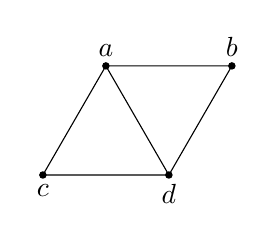
\begin{tikzpicture}[scale=0.4]
  \coordinate[label=above:$a$] (a) at (2,3.464);
  \coordinate[label=above:$b$] (b) at (6,3.464);
  \coordinate[label=below:$c$] (c) at (0,0);
  \coordinate[label=below:$d$] (d) at (4,0);

  \draw (a) -- (d) -- (c) -- cycle;
  \draw (d) -- (b) -- (a);
  \draw[black,fill] (a) circle [radius=0.1cm] ;
  \draw[black,fill] (b) circle [radius=0.1cm] ;
  \draw[black,fill] (c) circle [radius=0.1cm] ;
  \draw[black,fill] (d) circle [radius=0.1cm] ;
\end{tikzpicture} &
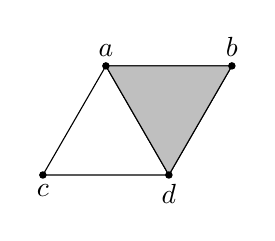
\begin{tikzpicture}[scale=0.4]
  \coordinate[label=above:$a$] (a) at (2,3.464);
  \coordinate[label=above:$b$] (b) at (6,3.464);
  \coordinate[label=below:$c$] (c) at (0,0);
  \coordinate[label=below:$d$] (d) at (4,0);

  \draw (a) -- (d) -- (c) -- cycle;
  \draw (d) -- (b) -- (a);
  \draw[fill=gray!50] (a) -- (d) -- (b) -- cycle;
  \draw[black,fill] (a) circle [radius=0.1cm] ;
  \draw[black,fill] (b) circle [radius=0.1cm] ;
  \draw[black,fill] (c) circle [radius=0.1cm] ;
  \draw[black,fill] (d) circle [radius=0.1cm] ;
\end{tikzpicture} \\
\hline
$\emptyset = K_0$ & $K_1$ & $K_2$ & $K_3$ & $K_4 = K$ \\
\hline
\end{tabular}
}
\caption{A filtration of $K$}
\label{fig:filtration}
\end{figure}

\begin{example}
Figure~\ref{fig:filtration} shows one possible filtration of our space $K$.
\end{example}

A practical source of filtered complexes comes from point cloud data.

\begin{definition}
Let $(X, d_X)$ be a metric space. The \emph{Vietoris-Rips complex of $X$} with parameter $\alpha$ is the simplicial complex with vertex set $X$ and simplices given by subsets of $X$ that are mutually no more than $\alpha$ distance apart. In other words,
\begin{align*}
  \mathbf{VR}(X, \alpha) = \{ \sigma \subseteq X \st d_X(x_i, x_j) \leq \alpha \text{ for all } x_i, x_j \in \sigma \}.
\end{align*}
\end{definition}


\begin{figure}
\makebox[\linewidth]{
\newcommand{\vrcomplex}[2][0.5]{
\begin{center}
\begin{tikzpicture}[scale=#1]
  \coordinate (a) at (2,3.3);
  \coordinate (b) at (7,4);
  \coordinate (c) at (0,0);
  \coordinate (d) at (3.5,0);

\clip (-3, -3) rectangle (10, 7);
\draw[white, fill, opacity=0] (-3, -3) rectangle (10, 7);

  \draw[black,fill] (a) circle [radius=0.1cm];
  \draw[black,fill] (b) circle [radius=0.1cm];
  \draw[black,fill] (c) circle [radius=0.1cm];
  \draw[black,fill] (d) circle [radius=0.1cm];

\draw[cyan, fill, opacity= 0.3] (a) circle (#2cm);
\draw[black] (a) circle (#2cm);
\draw[cyan, fill, opacity= 0.3] (b) circle (#2cm);
\draw[black] (b) circle (#2cm);
\draw[cyan, fill, opacity= 0.3] (c) circle (#2cm);
\draw[black] (c) circle (#2cm);
\draw[cyan, fill, opacity= 0.3] (d) circle (#2cm);
\draw[black] (d) circle (#2cm);
\end{tikzpicture}
\end{center}
}

\newcommand{\annuluscomplex}[1]{
\begin{figure}
\noindent\makebox[\textwidth]{%
\begin{tikzpicture}[scale=0.3]
%\begin{tikzpicture}[remember picture, overlay, scale=0.3]
%\tikzset{shift={(current page.center)},yshift=0cm}
\clip (-20, -10) rectangle (20, 10);
\draw[white, fill, opacity=0] (-20, -10) rectangle (20, 10);

\def\points{8.092593/0.134148,8.447231/0.949326,7.658496/1.144397,8.815373/2.177150,8.398666/2.076670,
9.006517/3.977381,7.520945/2.129330,6.698849/2.255754,5.807683/2.718666,7.062904/3.015901,
7.278569/4.457003,5.898714/4.987420,4.562342/5.118081,4.727490/6.667248,4.005391/6.592861,
3.983471/7.332549,4.038059/8.096364,3.859597/8.469849,3.195593/6.353141,3.981205/6.389805,
2.429519/8.228017,3.216939/6.555953,1.802313/7.954675,2.259787/8.041740,-0.397224/9.074358,
0.401439/7.953553,-1.266806/7.655207,-0.623094/8.432865,-1.053032/8.554193,-3.427812/7.770895,
-3.352173/7.103145,-3.918641/6.328826,-3.049035/7.426226,-2.966824/6.214639,-4.897973/5.293921,
-4.003319/7.130895,-4.712890/5.274353,-7.091653/5.528760,-5.655604/5.897540,-6.628111/4.522957,
-5.341439/5.245499,-8.360414/3.793542,-7.223336/4.216060,-7.555821/3.819587,-7.634792/2.563077,
-6.865465/0.812593,-8.336023/1.255058,-7.045293/1.036940,-8.049704/0.071260,-9.388684/-0.655015,
-8.968349/0.711340,-7.298501/-0.970684,-7.979053/-0.100698,-8.845275/-2.088935,-8.152570/-1.446517,
-7.195373/-3.045787,-8.253632/-2.281902,-6.395403/-2.900581,-7.635319/-4.477232,-5.337140/-5.388422,
-6.981240/-4.074050,-5.165616/-3.986240,-6.545813/-6.218857,-5.876391/-5.532203,-6.071537/-6.550160,
-4.202732/-5.660057,-3.449910/-6.121640,-3.412754/-8.166190,-3.313574/-6.292893,-2.183215/-6.090390,
-1.688938/-7.667467,-1.101403/-6.677577,-0.731159/-7.654493,0.701523/-9.010581,-1.000123/-8.899405,
1.008500/-8.270074,0.095397/-7.204591,0.247374/-6.901711,2.207983/-6.904603,2.225776/-8.183645,
2.731266/-7.370991,3.809154/-8.507204,4.589025/-8.216510,3.768458/-7.888926,5.126484/-5.980651,
4.792897/-6.223641,6.453863/-6.807602,6.788623/-5.535615,5.397679/-6.199476,6.782544/-6.078341,
6.976776/-3.272989,7.113013/-3.707895,8.333235/-2.149533,6.721281/-2.383298,7.054791/-2.247895,
6.601233/-1.062992,9.174918/-0.376968,8.372294/0.453995,7.922283/-2.005824,8.417951/1.096316}

\foreach \x / \y in \points{
\draw[cyan, fill, opacity=0.3] (\x,\y) circle (#1cm);
}

\foreach \x / \y in \points{
\draw[gray] (\x,\y) circle (#1cm);
}

\foreach \x / \y in \points{
\draw[black,fill] (\x,\y) circle [radius=0.1cm];
}
\end{tikzpicture}
}
\end{figure}
}
}
\caption{The Vietoris-Rips complex of a set of points for a particular $\alpha$}
\label{fig:vrcomplex}
\end{figure}

\begin{example}
The simplest example is a set of points $P \subset \R^n$ endowed with the ordinary Euclidean metric. Figure~\ref{fig:vrcomplex} shows a set of points $P \subset \R^2$. A ball is placed around each point. On the right hand side we note the subsets of $P$ in which the ball around any point contains the entire subset. These subsets become our simplices. 
\end{example}

Clearly, if a simplex $\sigma \in \mathbf{VR}(X, \alpha')$ then $\sigma \in \mathbf{VR}(X, \alpha)$ for any $\alpha \geq \alpha'$. Again, we get a filtration $\{\mathbf{VR}(X, \alpha)\}_{\alpha \in \mathbf{R}}$.

\subsection{Multisets}

One of the main objects we will define in this work is the \emph{persistence diagram}, a multiset of points in the plane. Informally, a multiset is a set in which elements are permitted to appear more than once.

\begin{definition}
A \emph{multiset} is a pair $\A = (A, m)$, where $A$ is an ordinary set and $m : A \to \N$ is the \emph{multiplicity function}. For any $a \in A$, $m(A) \in \N$ is the number of times $a$ appears in $\A$.
\end{definition}

It will be convenient to think of a multiset $\A$ as an ordinary set $A$, where we artificially distinguish elements with multiplicity $m(a) > 1$ by pretending each is labelled $a_1, a_2, \dots$, and so on. In what follows, we will often take this perspective without comment.
\section{Standard Persistent Homology}
\label{section-standard}

We begin by describing persistent homology over a field for finite simplicial complexes. These conditions allow a complete characterisation of the persistent homology of a filtration via simple combinatorial objects called barcodes. In practice, because our data is finite, we always deal with finite simplicial complexes. Algorithms exist to compute the barcode of a filtration of a simplicial complex.

\subsection{Persistent homology groups}

A filtration is a way of gradually building up a topological space. We can extend our definition of homology to apply to each intermediate space in a filtration. Because our filtration is finite, without loss of generality we consider filtrations indexed by the natural numbers.

First, fix a dimension $n$ and consider all homology to be done at this dimension. Let $K$ be a filtration and let $H_i$ denote the homology of the space $K_i$.

If we wish to use a filtration to find topological features of a space, we might consider, for example, the sequence of Betti numbers produced by moving up the filtration. Unfortunately, from these alone there is no way to distinguish true features of the space from the noise caused by our construction of the filtration.

In any filtration there are inclusion maps $\iota_i^j : K_i \to K_j$ for any $i \leq j$. By Theorem~\ref{homology-functor}, each induces a homomorphism $\eta_i^j : H_i \to H_j$. When we move to the right in this sequence, we could gain homology classes or lose some as they become trivial or merge together.

The idea behind persistence is that any significant topological feature of the data should exist along a large interval of the filtration. This leads us to define the persistent homology groups of our filtration, which will represent homology classes in each space that still exist some number of spaces later in the filtration.

\begin{definition}[Persistent homology]
Let $K_i$ be a filtration. The \emph{persistent homology groups of $K$}, denoted $H_i^j$, are the images of the induced homomorphisms $\eta_i^j$.
\end{definition}

These groups consist of the homology classes of $K_i$ that are still ``alive'' in $K_j$. An alternative definition is to factor out the cycle group of $K_i$ by the boundary group of $K_j$:
\begin{align*}
H_i^j = Z_i / (B_j \cap Z_i).
\end{align*}
Both $B_j$ and $Z_i$ are subgroups of $C_j$, so the intersection $B_j \cap Z_i$ is well-defined.

We can also track the lifetime of an individual homology class. Let $\gamma \in H_i$. We say $\gamma$ is \emph{born at $K_i$} if it first appears in $K_i$, i.e., $\gamma \notin H_{i-1}^i$. The class \emph{dies entering $K_j$} if it merges with an older class when we move from $K_{j-1}$ to $K_j$. That is,
\begin{enumerate}
\item $\eta_i^{j-1}(\gamma) \notin H_{i-1}^{j-1}$ ($\gamma$ in $K_{j-1}$ is not the image of a class in $K_{i-1}$); but,
\item $\eta_i^j(\gamma) \in H_{i-1}^j$ ($\gamma$ in $K_{j}$ is the image of a class in $K_{i-1}$).
\end{enumerate}

The \emph{lifetime} of a homology class $\gamma$ is the half-open interval $[i, j)$, where $\gamma$ is born at $K_i$ and dies entering $K_j$. If $\gamma$ is born at $K_i$ but then never dies, its lifetime is $[i, \infty)$.

\begin{example}
Consider the filtration given earlier as Figure~\ref{fig:filtration}. The homology class $\sigma = [a, b] + [b, d] - [a, d]$ is born at stage $K_3$, as it is not the image of a homology class in any earlier $K_i$. It dies one step later in $K_4$, as the class becomes trivial. The lifetime of $\sigma$ is therefore $[3, 4)$.
\end{example}

\subsection{Persistence modules}

At this point it is not clear whether we can get a succinct description of the persistent homology of a filtration. In their foundational paper, Zomorodian and Carlsson \cite{zomorodian2005computing} showed that a description exists for finite simplicial complexes when the homology coefficient ring is a field.

Intuitively, computing persistent homology requires us to find compatible bases for $H_i$ and $H_j$. We begin by constructing one large structure that contains the homology groups for all steps in the filtration.

\begin{definition}
A \emph{persistence module} $\mathcal{M}$ is a family of $R$-modules $\{ M_i \}_{i \geq 0}$ together with module maps $\varphi_i : M_i \to M_{i+1}$.
\end{definition}

The set of homology groups $H_i$ form a persistence module, with the maps $\varphi_i$ induced by the inclusion maps $K_i \to K_{i+1}$.

Given a persistence module, we can construct a single graded module that contains the same data. Let $\mathcal{M} = \{M_i, \varphi_i\}$ be a persistence module over the ring $R$. Now define the graded module over $R[t]$:
\begin{align*}
  \alpha(\mathcal{M}) = \bigoplus_{i=0}^\infty M_i,
\end{align*}
where the action of $R$ is just the action on each component, and the action of $t$ is
\begin{align*}
t \cdot (m_0, m_1, m_2, \dots) = (0, \varphi_0(m_0), \varphi_1(m_1), \varphi_2(m_2), \dots).
\end{align*}

In homology terms, multiplication by $t$ moves a homology class up the filtration by one. If some homology class $\gamma$ exists in $K_i$, then $t \cdot \gamma$ is an element of $K_{i+1}$.

\begin{definition}
A graded module $R[t]$ is of \emph{finite type} if each $M_n$ is finite dimensional over $R$.
\end{definition}

Because our filtration is finite, its homology is also finite and therefore the graded $R[t]$ module will be of finite type.

\begin{theorem}[Correspondence]
The map $\alpha$ is a one-to-one correspondence between the set of persistence modules over $R$ and the set of graded modules of finite type over $R[t]$.
\end{theorem}
\begin{proof}
We construct an inverse to $\alpha$ in the obvious way. If $G$ is a graded module of finite type over $R[t]$, let $M_i$ be the submodule of $G$ with grading $i$ considered as a $R$-module and set $\varphi_i(a) = t \cdot a \in M_{i+1}$.
\end{proof}

From this we learn there is little hope for a simple classification of persistence modules when the ground ring is not a field. Even in the simple case of $R=\mathbf{Z}$, $\mathbf{Z}[t]$-modules are known to be extremely difficult to classify.

When $R$ is a field $\mathbf{k}$, the graded ring $\mathbf{k}[t]$ is a PID, so we can classify the persistence modules using Theorem~\ref{thm:graded-pid-structure}, the structure theorem for graded modules over PIDs. The only graded ideals of $\mathbf{k}[t]$ are homogeneous of the form $\langle t^n \rangle$, so
\begin{align*}
\alpha(\mathcal{M}) \cong \left( \bigoplus_{i=1}^n \Sigma^{\alpha_i} \mathbf{k}[t] \right) \oplus \left( \bigoplus_{i=1}^m \Sigma^{\beta_i} \mathbf{k}[t] / \langle t^{n_i} \rangle \right).
\end{align*}

Remember that $\Sigma^k$ represents an upward shift of $k$ steps in the grading.

This decomposition holds the description for persistence that we seek. In the first sum, the free part, each summand gives a class $\gamma$ that first appears at time $\alpha_i$, and $t \cdot \gamma, t^2 \cdot \gamma, \dots$ remain nonzero for all steps in the filtration after that. This corresponds to a persistence interval of $[\alpha_i, \infty)$.

In the second sum, the torsion part, a class $\tau$ first appears at time $\beta_i$, and exists as $t \cdot \tau, t^2 \cdot \tau, ..., t^{n_i-1} \cdot \tau$. After this, $t^{n_i}$ becomes zero, so our homology class is mapped to zero at time $\beta_i + n_i$. This gives us an interval $[\beta_i, \beta_i + n_i)$.

These sets of intervals are known as \emph{barcodes}. More precisely:

\begin{definition}
A \emph{barcode} is a finite multiset of ordered pairs $(i, j)$, with $0 \leq i < j$, and $i, j \in \mathbb{Z} \cup \{\infty\}$.
\end{definition}

The barcode exactly determines the structure of a $\mathbf{k}[t]$-module, so we can restate the correspondence as follows:

\begin{corollary}
There is a bijective correspondence between barcodes and persistence modules of finite type over a field.
\end{corollary}

\begin{example}
Let us return to the filtration shown in Figure~\ref{fig:filtration} and compute the barcode for the 0-dimensional homology. The space $K_1$ introduces two new components, so two new homology classes. Both classes are mapped into the same component in $K_2$, so one of the classes dies entering $K_2$. An additional class is born in $K_2$, which then joins the rest of the  space in $K_3$. The barcode is therefore $\{[1,2), [1, \infty), [2, 3)\}$.

Similarly, two 1-dimensional homology classes are created in $K_3$. In $K_4$, one of these becomes trivial. The barcode is then $\{[3, 4), [3, \infty) \}$.
\end{example}

Barcodes can be represented pictorially by simply plotting each interval $[p, q)$ as a point $(p, q)$ in the plane. This set of points must lie above the line $x = y$. Features with short lifetimes will correspond to points that lie close to the diagonal.

\begin{figure}
\centering
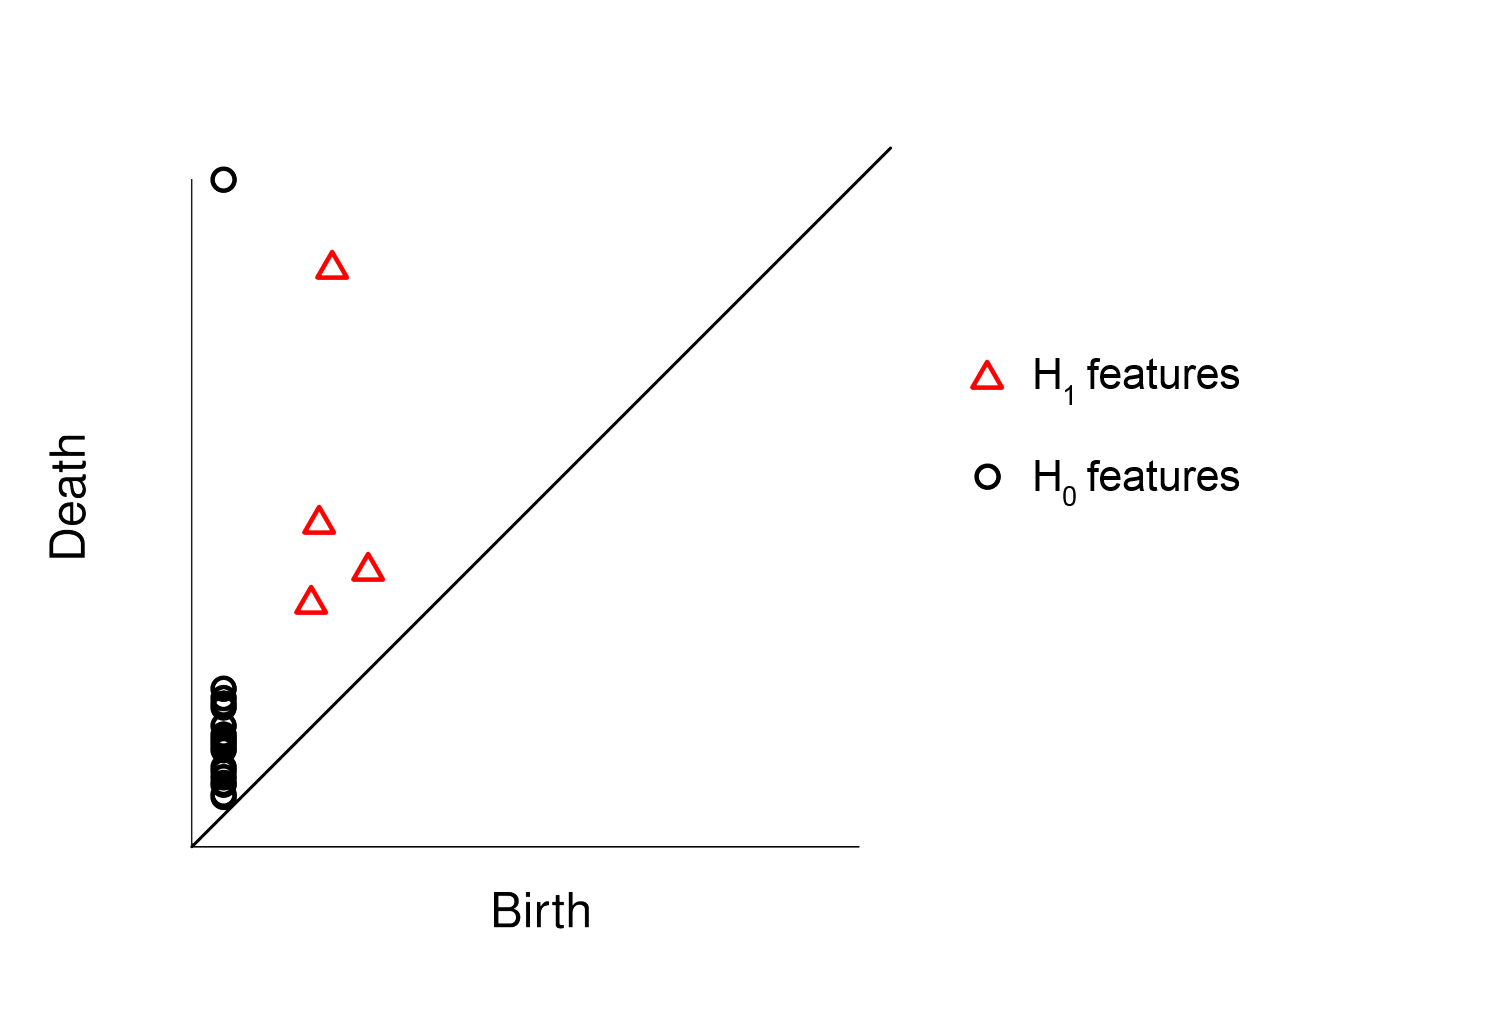
\includegraphics[scale=0.3]{diagram.png}

\caption{A sample persistence diagram}
\label{fig:examplediagram}
\end{figure}

\subsection{Algorithms}

Zomorodian and Carlsson also provide an algorithm to systematically calculate the barcode of an input filtration. Appendix~\ref{code-appendix} contains a Haskell implementation of the algorithm, completed as part of this project. Haskell was chosen as it is well suited for defining mathematical objects such as simplices, groups, vector spaces, and so on.

The algorithm has since been improved in a number of ways. Most notably, calculating persistent cohomology \cite{de2011dualities} has been shown to have much better performance in practice. Poincar\'e duality implies that over $\mathbb{Z}/2\mathbb{Z}$, the barcodes produced this way are the same as would be produced by persistent homology.
\section{Persistence Modules}
\label{section-modules}

In its first incarnation, persistent homology was an algorithm that given a filtration, directly produced a barcode. The previous section shows there is an intermediate object, the persistence module, that captures all the important algebraic data contained in the filtration. In this section we give a more general definition of persistence modules and derive some of their basic properties.

As before, we fix a field $\mathbf{k}$ with all vector spaces over this field.

\begin{definition}
Let $\mathbf{P}$ be a partially ordered set. A \emph{persistence module $\V$ over $\mathbf{P}$} is a collection of vector spaces $\{V_t \st t \in \mathbf{P}\}$ and linear maps $\{v_s^t \st s, t \in \mathbf{P}, s \leq t\}$ such that for all $r \leq s \leq t$, we have $v_r^t = v_s^t \circ v_r^s$. 
\end{definition}

These linear maps are often called the \emph{structure maps} of $\V$. We recover the definition of the previous section when we set $P = \mathbf{N}$, the natural numbers. In what follows, we will mainly be interested in persistence modules over the real numbers $\R$. If $K$ is a filtration, we will write $H(K)$ for the persistence module induced by $K$.

\begin{definition}
If $\V$ is a persistence module over $\T$, and $\mathbf{P} \subset \T$, then the \emph{restriction of $\V$ to $\mathbf{P}$}, written $\V_{\mathbf{P}}$, is the persistence module obtained by forgetting the spaces and maps that lie outside $\mathbf{P}$. To be specific, $\V_{\mathbf{P}}$ is the persistence module with spaces and structure maps
\begin{align*}
(V_{\mathbf{P}})_t & = V_t \\
(v_{\mathbf{P}})_s^t &= v_s^t
\end{align*}
for $s, t \in \mathbf{P}$.
\end{definition}

As with any algebraic object, we also require a notion of a mapping between persistence modules. 

\begin{definition}
A \emph{homomorphism} $\Phi : \U \to \V$ between two persistence modules over $\mathbf{P}$ is a collection of linear maps $\{ \phi_t : U_t \to V_t \st t \in \mathbf{P} \}$ such that the following diagram commutes for all $s \leq t$. 

\begin{displaymath}
\xymatrix{
U_s \ar[d]_{\phi_s} \ar[r]^{u_s^t} & U_t \ar[d]^{\phi_t}\\
V_s \ar[r]^{v_s^t} & V_t
}
\end{displaymath}

We compose morphisms in the obvious way. Suppose we have $\Phi : \U \to \V$ and $\Psi : \V \to \W$, where $\Phi = \{\phi_t\}$ and $\Psi = \{\psi_t\}$. Then composition $\Psi \Phi$ is given by $\Psi \Phi = \{ \psi_t \phi_t \}$. To see that the relevant diagram commutes, notice that
\begin{displaymath}
\xymatrix{
U_s \ar[d]_{\phi_s} \ar[r]^{u_s^t} & U_t \ar[d]^{\phi_t}\\
V_s \ar[d]_{\psi_s} \ar[r]^{v_s^t} & V_t \ar[d]^{\psi_t}\\
W_s \ar[r]^{w_s^t} & W_t
}
\end{displaymath}
commutes, as both the top and bottom squares do.

The \emph{identity} and \emph{zero} homomorphisms are just the identity and zero maps at each point. The \emph{image}, \emph{kernel} and \emph{cokernel} of a homomorphism are also defined pointwise with the canonical structure maps. For example, the kernel of $\Phi$ is given by:
\begin{align*}
\text{Ker}(\Phi)_t &= \ker(\phi_t) \\
\ker(\Phi)_s^t &= u_s^t|_{\ker(\phi_t)}.
\end{align*}
\end{definition}

For convenience, we also define $\Hom(\U, \V) = \{ \text{homomorphisms } \U\to\V \}$ and $\End(\V) = \Hom(\V, \V)$.

\subsection{Interval modules}

The simplest examples of persistence modules are the interval modules. These will correspond to points in our barcode.

\begin{definition}
Let $J \subseteq \R$ be an interval. Then $\I^J$ is defined to be the persistence module with spaces
\begin{align*}
I_t = \begin{cases}
\mathbf{k} & \text{if } t \in J; \\
0 & \text{otherwise}
\end{cases}
\end{align*}
and maps
\begin{align*}
i_s^t = \begin{cases}
1 & \text{if } t, s \in J; \\
0 & \text{otherwise.}
\end{cases}
\end{align*}
\end{definition}

Over $\R$, providing the endpoints is not enough to determine the interval as the interval could be either closed or open on each end. To simplify the notation, we describe the endpoints of intervals using \emph{decorated real numbers}: real numbers with a superscript $+$ or $-$ annotation. For finite intervals, these decorated numbers are interpreted as follows:
\begin{align*}
(p^-, q^-) &= [p, q); \\
(p^-, q^+) &= [p, q]; \\
(p^+, q^-) &= (p, q); \\
(p^+, q^+) &= (p, q]. 
\end{align*}
We also use the natural ordering
\begin{align*}
p^- < p < p^+ < q^- < q < q^+
\end{align*}
whenever $p < q$. If the annotation is unknown or unimportant, an asterisk is used. The expression $(p^*, q^*)$ with $p^* < q^*$ thus represents an arbitrary interval. 

\subsection{Interval decompositions}

We would like to be able to analyse persistence modules by decomposing them into interval modules. There is a natural definition for the sum of two persistence modules.

\begin{definition}
The \emph{direct sum} $\W = \U \oplus \V$ of two persistence modules is the persistence module with spaces and structure maps:
\begin{align*}
W_t = U_t \oplus V_t \\
w_s^t = u_s^t \oplus v_s^t.
\end{align*}
\end{definition}

This definition generalises in the obvious way to direct sums with arbitrary summands.

We say that a persistence module $\W$ is \emph{indecomposable} if the only decompositions of the form $\W = \U \oplus \V$ are $\W \oplus 0$ and $0 \oplus \W$.

\begin{proposition}
Interval modules are indecomposable.
\end{proposition}
\begin{proof}
Let $\I$ be an interval module with decomposition $\I = \U \oplus \V$. Then the projection maps onto $\U$ and $\V$ are idempotent elements of $\End(\I)$. Any endomorphism of $\I$ acts on each $I_t$ by scalar multiplication and, as the structure maps are commutative, the scalar must be the same for each $t$. Therefore, $\End(\I) = \mathbf{k}$, and the only idempotents are $0$ and $1$. Our projection maps are therefore either $0$ or $1$, so we must have one map $0$ and the other map $1$ as required.
\end{proof}

If our persistence module is decomposable into interval modules, the following theorem guarantees that the decomposition is unique up to reordering. The theorem is the analogue of the Krull-Schmidt theorem \cite{azumaya1950corrections} for group decompositions, which has since been generalised to many algebraic objects for which `decomposition' makes sense.

\begin{theorem}[Krull-Schmidt-Azumaya]
Suppose a persistence module $\V$ is decomposable into interval modules in two different ways:
\begin{align*}
\V = \bigoplus_{l \in L} \I^{J_l} = \bigoplus_{m \in M} \I^{K_m}.
\end{align*}
Then $|L| = |M|$, and there exists a permutation $\pi$ such that $J_l = K_{\pi(l)}$ for all $l \in L$.
\end{theorem}
\begin{proof} Here we specialise an argument given by Barot \cite{barot2006representations} for decompositions with finitely many summands. Let $\Phi : \V \to \W$ be an isomorphism, and let $\V = \V_1 \oplus \dots \oplus \V_n$ and $\W = \W_1 \oplus \dots \oplus \W_m$ be interval decompositions.

We can write $\Phi$ as a matrix $\Phi = (\Phi_{ji})$ where each $\Phi_{ji}$ is a homomorphism $\V_i \to \W_j$. Similarly, we can write $\Phi^{-1} = \Psi$ as a matrix $(\Psi_{ji})$. Consider: 
\begin{align*}
\mathbf{1}_{\V_1} = (\Psi \Phi)_{11} = \sum_{l=1}^j \Psi_{1l} \Phi_{l1}.
\end{align*}
As the left-hand side is nonzero, one of the summands $\Psi_{1l} \Phi_{l1}$ must be nonzero. Without loss of generality, assume $\Psi_{11} \Phi_{11}$ is nonzero and therefore invertible. Because $\V_1$ and $\W_1$ are indecomposable, $\Psi_{11}$ and $\Phi_{11}$ are onto and hence are themselves invertible.

Now we construct two change of basis matrices:
\begin{align*}
\alpha = \begin{pmatrix}
\mathbf{1}_{\W_1} & 0 & \cdots & 0 \\
-\Phi_{21} \Phi_{11}^{-1} & \mathbf{1}_{\W_2} & \cdots & 0 \\
\vdots & \vdots & \ddots & \vdots \\
-\Phi_{m1} \Phi_{11}^{-1} & 0 & \cdots & \mathbf{1}_{\W_m} \\
\end{pmatrix} \quad 
\beta = \begin{pmatrix}
\mathbf{1}_{\V_1} & -\Phi_{11}^{-1} \Phi_{12} & \cdots & -\Phi_{11}^{-1} \Phi_{1n} \\
0 & \mathbf{1}_{\V_2} & \cdots & 0 \\
\vdots & \vdots & \ddots & \vdots \\
0 & 0 & \cdots & \mathbf{1}_{\V_m} \\
\end{pmatrix}
\end{align*}
and set $\Phi' = \alpha \Phi \beta$. Then $\Phi' : \V \to \W$ is another isomorphism of the form $\Phi' = \begin{pmatrix}
\Phi_{11} & 0\\
0 & \Lambda
\end{pmatrix}$ 
with $\Lambda : \bigoplus_{i=2}^n \V_i \to \bigoplus_{j=2}^m \W_j$ an isomorphism of the remaining summands. The result follows by induction.

The infinite case is much harder, and we refer the reader to Azumaya \cite{azumaya1950corrections}. To apply this theorem, the indecomposable modules must satisfy a certain condition: that $\End(\I)$ be a `local' ring. As $\End(\I) = \mathbf{k}$ is a field and all fields are local, this condition is satisfied. In the finite case above, this property is required to conclude that one of $\Psi_{1l} \Phi_{l1}$ is invertible.
\end{proof}

We saw in the previous section that if our indexing set is a finite subset of $\R$ and the vector spaces are pointwise finite dimensional then the persistence module decomposes into interval modules. A number of researchers have independently shown that we can drop the restriction on the dimension of the vector spaces:

\begin{theorem}[Auslander \cite{auslander1974representation}]
Let $\T$ be a finite, totally ordered set. Then any persistence module over $\T$ decomposes as a sum of interval modules.
\label{thm-finite-decomposition}
\end{theorem}

The theorem is false for arbitrary persistence modules. The following module provides a counterexample.

\begin{example}[Webb \cite{chazal2012structure}]
Let $\V$ be the persistence module over the non-positive integers with spaces
\begin{align*}
V_0 &= \{ \text{sequences of real numbers } (x_1, x_2, \dots) \}\\
V_{-n} &= \{ \text{sequences with } x_1 = \dots = x_n = 0 \} \text{ for } n \geq 1
\end{align*}
and structure maps the natural inclusions $v_{-m}^{-n}$ for $m \geq n$.

First note that $\dim(V_0)$ is uncountable. Any vector in a vector space must be able to be written as a linear combination of finitely many basis elements. It can be proven that no countable basis exists for sequences of real numbers.

Now, because the structure maps are all injective, the intervals in an interval decomposition must all be of the form $[-n, 0]$. Since $\dim(V_{-n}/V_{-n-1}) = 1$, each $[-n,0]$ occurs with multiplicity 1. This implies that $\V \cong \bigoplus_{n\geq0} \I[-n, 0]$, which contradicts the fact that $\dim(V_0)$ is uncountable.
\end{example}

\subsection{Quiver calculations}

In this section, we introduce some notation that will simplify future calculations. We then prove some basic properties of persistence modules over finite sets using this tool. 

A persistence module $\V$ over a finite set $a_1 < a_2 < \dots < a_n$ can be thought of as a diagram of vector spaces:
\begin{align*}
V_{a_1} \to V_{a_2} \to \dots \to V_{a_n}
\end{align*}

Diagrams of this sort are also known as `quiver representations of type $A_n$'. Theorem~\ref{thm-finite-decomposition} states that such a persistence module decomposes as a sum of interval modules. Because we are over a finite set, we can represent such interval modules pictorially. We use filled circles to represent indices where the module is $\mathbf{k}$ and open circles for where the module is 0.

Consider the finite set $a < b < c$. There are precisely six interval modules over $\{a, b, c\}$:
\begin{align*}
\I[a, a] &= \qon{a} \qem \qoff{b} \qem \qoff{c} \qquad \I[a, b] = \qon{a} \qem \qon{b} \qem \qoff{c} \qquad \I[a, c] = \qon{a} \qem \qon{b} \qem \qon{c}\\
\I[b, b] &= \qoff{a} \qem \qon{b} \qem \qoff{c} \qquad \I[b, c] = \qoff{a} \qem \qon{b} \qem \qon{c} \\
\I[c, c] &= \qoff{a} \qem \qoff{b} \qem \qon{c} 
\end{align*}

\begin{definition}
Let $\V$ be a persistence module over $\R$ and $\T \subset \R$ a finite subset. Given an arbitrary interval module 
\begin{align*}
\I = \: \qoff{r} \qem \dots \qem \qoff{} \qem \qon{a} \qem \dots \qem \qon{b} \qem \qoff{} \qem \dots \qem \qoff{s}
\end{align*}
on $\T$, we write
\begin{align*}
\langle \I \st \V_\T \rangle \text{ or } \langle \qoff{r} \qem \dots \qem \qoff{} \qem \qon{a} \qem \dots \qem \qon{b} \qem \qoff{} \qem \dots \qem \qoff{s} \st \V \rangle \text{ or } \langle [a, b] \st \V_\T \rangle
\end{align*}
for the multiplicity of $\I$ in the interval decomposition of $\V_\T$. We will omit $\V_\T$ when the persistence module and indexing sets are clear.
\end{definition}

\begin{example}
Consider one of the structure maps $v_s^t : V_s \to V_t$. Then:
\begin{align*}
\langle \qon{s} \qem \qon{t} \st \V \rangle = \rank(v_s^t).
\end{align*}
\end{example}

If our persistence module is the direct sum of simpler modules, the multiplicity of an interval is simply the sum of the multiplicities in these simpler modules.

\begin{proposition}
\label{quiver-direct-sums}
Let $\V$ be written as a direct sum
\begin{align*}
\V = \bigoplus_{i \in I} \V^i.
\end{align*}
Then
\begin{align*}
\langle [a, b] \st \V_\T \rangle = \sum_{i\in I} \langle [a, b] \st \V_\T^i \rangle
\end{align*}
for any interval module $[a, b]$ in a finite indexing set $\T$.
\end{proposition}
\begin{proof}
Individually decompose the $\V_\T^i$ into interval modules as in Theorem~\ref{thm-finite-decomposition}. The sum of all these interval modules is a decomposition of $\V_\T$. The multiplicity of $[a, b]$ in $\V_\T$ is then the sum of the multiplicities in $\V_\T^i$.
\end{proof}

The final property of the multiplicities we discuss here is the so called `restriction principle'. This allows us to relate the multiplicities of different finite restrictions of the same module.

\begin{proposition}
Let $\S$ and $\T$ be finite index sets with $\S \subset \T$. For any interval module $\I$ over $\S$,
\begin{align*}
\langle \I \st \V_\S \rangle = \sum_\J \langle \J \st \V_\T \rangle
\end{align*}
where $\J$ runs over all interval modules in $\T$ that restrict to $\I$ over $\S$.
\end{proposition}

\begin{example}
Consider the finite indexing set $a < p < b < q < c$. Then:
\begin{align*}
\langle \qoff{a} \qem \qno \qem \qon{b} \qem \qno \qem \qon{c} \rangle = \langle \qoff{a} \qem \qoff{p} \qem \qon{b} \qem \qon{q} \qem \qon{c} \rangle + \langle \qoff{a} \qem \qon{p} \qem \qon{b} \qem \qon{q} \qem \qon{c} \rangle
\end{align*}
\end{example}

\begin{proof}
Consider an interval decomposition of $\V_\T$. This restricts to an interval decomposition of $\V_\S$. Instances of $\I$ in this decomposition appear precisely when the interval $\J$ restricts to $\I$ over $\S$.
\end{proof}


\section{Persistence Diagrams}
\label{section-diagrams}

In this section we define the diagram of a persistence module over $\R$, generalising the barcode of standard persistent homology. If a persistence module $\V$ is decomposable into interval modules, we can use the obvious definition: the multiset in $\R^2$ with a point at $(p, q)$ for each interval $\I(p^*, q^*)$. When $\V$ does \emph{not} decompose into interval modules, we will have to work a little harder.

The strategy is as follows. To every persistence module over $\R$ we associate an `r-measure': a function that assigns every rectangle in $\R^2$ an integer measure. We then show there is a bijection between the appropriate classes of r-measures and multisets in $\R^2$.

\subsection{Abstract r-measures}

First we define r-measures and derive some of their basic properties.

\begin{definition}
Let $\mathcal{D}$ be a subset of $\R^2$. We define $\Rect(\mathcal{D})$ to be the set of closed rectangles lying inside $\mathcal{D}$, i.e., 
\begin{align*}
\Rect(\mathcal{D}) = \{ [a, b] \times [c, d] \subset \mathcal{D} \st a < b \text{ and } c < d \}
\end{align*}
An \emph{r-measure} on $\mathcal{D}$ is a function $\mu : \Rect(\mathcal{D}) \to \{0, 1, 2, \dots \} \cup \{\infty\}$ that is additive under horizontal and vertical splits:
\begin{align*}
\mu([a, b] \times [c, d]) &= \mu([a, p] \times [c, d]) + \mu([p, b] \times [c, d])\\
\mu([a, b] \times [c, d]) &= \mu([a, b] \times [c, q]) + \mu([a, b] \times [q, d])
\end{align*}
for $a < p < b$ and $c < q < d$. Figure~\ref{fig:rmeasure} shows how to interpret these equations pictorially.

\begin{figure}[!htb]
\centering
\begin{tabular}{c c c c}
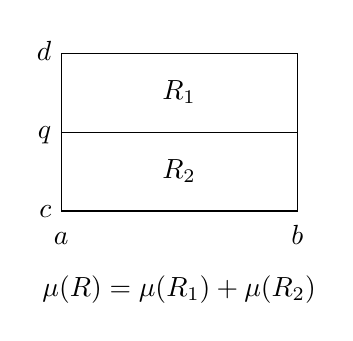
\begin{tikzpicture}[scale=2]
  \coordinate (a) at (0,0);
  \coordinate (b) at (1.5, 0);
  \coordinate (c) at (1.5, 1);
  \coordinate (d) at (0, 1);
  
  \draw (a) rectangle (c);
  \path[draw] (0, 0.5) -- (1.5, 0.5);
  
  \draw (0.75,0.25) node {$\strut{R_2}$};  
  \draw (0.75,0.75) node {$\strut{R_1}$};    
  
  \draw (0,0) node[left] {$\strut{c}$};
  \draw (0,0.5) node[left] {$\strut{q}$};
  \draw (0,1) node[left] {$\strut{d}$};
  
  \draw (0,0) node[below] {$\strut{a}$};
  \draw (1.5,0) node[below] {$\strut{b}$};
  
  \draw (0.75, -0.5) node {$\mu(R) = \mu(R_1) + \mu(R_2)$};  
\end{tikzpicture} & & &
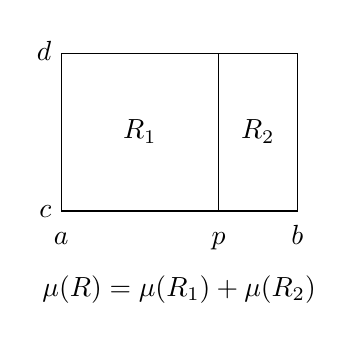
\begin{tikzpicture}[scale=2]
  \coordinate (a) at (0,0);
  \coordinate (b) at (1.5, 0);
  \coordinate (c) at (1.5, 1);
  \coordinate (d) at (0, 1);
  
  \draw (a) rectangle (c);
  \path[draw] (1, 0) -- (1, 1);
  
  \draw (0.5,0.5) node {$\strut{R_1}$};  
  \draw (1.25,0.5) node {$\strut{R_2}$};    
  
  \draw (0,0) node[left] {$\strut{c}$};
  \draw (0,1) node[left] {$\strut{d}$};
  
  \draw (0,0) node[below] {$\strut{a}$};
  \draw (1,0) node[below] {$\strut{p}$};
  \draw (1.5,0) node[below] {$\strut{b}$};
  
  \draw (0.75, -0.5) node {$\mu(R) = \mu(R_1) + \mu(R_2)$};  
\end{tikzpicture}
\end{tabular}
\caption{Horizontal and vertical splitting for r-measures}
\label{fig:rmeasure}
\end{figure}
\end{definition}

We will see that r-measures have many of the features of ordinary measures when restricted appropriately to rectangles in the plane.

\begin{proposition}[Finite additivity]
Let $\mu$ be an r-measure on $\mathcal{D}$. If a rectangle $R$ can be written as a union $R = R_1 \cup \dots \cup R_k$ of rectangles with disjoint interiors, then $\mu(R) = \mu(R_1) + \dots + \mu(R_k)$.
\end{proposition}
\begin{proof}
Let $R = [a, b] \times [c, d]$. By the vertical splitting property, the statement holds for any decomposition $R_i = [a_i, a_{i+1}] \times [c, d]$ with $a = a_1 < a_2 < \dots < a_n = b$. Similarly, by the horizontal splitting property, the statement holds for $R_i = [a, b] \times [c_j, c_{j+1}]$. with $c = c_1 < c_2 < \dots < c_m = d$.

By performing both types of splits, it follows that finite additivity holds for any `product' decomposition of the form $R_{ij} = [a_i, a_{i+1}] \times [c_j, c_{j+1}]$. Now for an arbitrary decomposition $R = R_1 \cup \dots \cup R_k$, decompose each component $R_i$ into the above form, so the entire decomposition also has the form of a `product'. The result follows.
\end{proof}

\begin{proposition}[Monotonicity]
If $R \subseteq S$ then $\mu(R) \leq \mu(S)$.
\end{proposition}
\begin{proof}
This follows from the above proposition, as $S$ must have a decomposition containing $R$ as a component. This can always be done with at most nine rectangles using the coordinates of $R$ as the locations of the splits, as suggested by Figure~\ref{fig:monotonicity}. Then:
\begin{align*}
\mu(S) &= \mu(R) + \mu(R_1) + \dots\\
&\geq \mu(R).
\end{align*}

\begin{figure}[!htb]
\centering
\begin{tikzpicture}[scale=3]
  \coordinate (a) at (0,0);
  \coordinate (b) at (1.5, 0);
  \coordinate (c) at (1.5, 1);
  \coordinate (d) at (0, 1);
  
  \coordinate (a') at (0.25, 0.25);
  \coordinate (c') at (1, 0.75);  
  
  \draw (a) rectangle (c);
  \draw[dashed] (0.25, 0) -- (0.25, 1);
  \draw[dashed] (1, 0) -- (1, 1);
  \draw[dashed] (0, 0.25) -- (1.5, 0.25);
  \draw[dashed] (0, 0.75) -- (1.5, 0.75);

  \draw (a') rectangle (c');
  
  \draw (0.62, 0.5) node {$\strut{R}$};
  \draw (0, 0.5) node[left] {$\strut{S}$};
\end{tikzpicture}

\caption{Splitting used in the proof of monotonicity}
\label{fig:monotonicity}
\end{figure}
\end{proof}

\begin{proposition}[Subadditivity]
If $R \subseteq R_1 \cup \dots \cup R_n$ then $\mu(R) \leq \mu(R_1) + \dots + \mu(R_n)$.
\end{proposition}
\begin{proof}
Let $\{a_i\}$ be the $x$-coordinates of the corners of every rectangle, and $\{c_j\}$ the $y$-coordinates. Subdivide every rectangle into tiles of the form $[a_i, a_{i+1}] \times [c_j, c_{j+1}]$. Every tile that comprises $R$ must belong to some $R_i$ and the result follows by additivity.
\end{proof}

\subsection{The persistence measure}

From any persistence module $\V$, we construct an r-measure that `counts' the points of the barcode of $\V$ that fall inside each rectangle. We can use this r-measure to construct a persistence diagram for \emph{any} persistence module, not only those that decompose into intervals.

Let $\H$ be the half-plane in $\R^2$ given by:
\begin{align*}
\H = \{ (p, q) \st p \leq q \}
\end{align*}

\begin{definition}
The \emph{persistence measure} of $\V$ is the function
\begin{align*}
\mu_\V(R) = \langle \qoff{a} \qem \qon{b} \qem \qon{c} \qem \qoff{d} \st \V \rangle,
\end{align*}
for any $R = [a, b] \times [c, d]$ with $a < b \leq c < d$.
\end{definition}

\begin{proposition}
$\mu_\V$ is a r-measure on $\H$.
\end{proposition}
\begin{proof}
We must show that $\mu_\V$ is additive under horizontal and vertical splitting. For horizontal splitting, let $a < p < b \leq c < d$. Then, by the restriction principle,
\begin{align*}
\mu_\V([a, b] \times [c, d]) &= \langle \qoff{a} \qem \qno \qem \qon{b} \qem \qon{c} \qem \qoff{d} \st \V \rangle\\
&= \langle \qoff{a} \qem \qon{p} \qem \qon{b} \qem \qon{c} \qem \qoff{d} \st \V \rangle + \langle \qoff{a} \qem \qoff{p} \qem \qon{b} \qem \qon{c} \qem \qoff{d} \st \V \rangle \\
&= \langle \qoff{a} \qem \qon{p} \qem \qno \qem \qon{c} \qem \qoff{d} \st \V \rangle + \langle \qno \qem \qoff{p} \qem \qon{b} \qem \qon{c} \qem \qoff{d} \st \V \rangle \\
&= \mu_\V([a, p] \times [c, d]) + \mu_\V([p, b] \times [c, d]).
\end{align*}

For vertical splitting, let $a < b \leq c < q < d$, then:
\begin{align*}
\mu_\V([a, b] \times [c, d]) &= \langle \qoff{a} \qem \qon{b} \qem \qon{c} \qem \qno \qem \qoff{d} \st \V \rangle\\
&= \langle \qoff{a} \qem \qon{b} \qem \qon{c} \qem \qoff{q} \qem \qoff{d} \st \V \rangle + \langle \qoff{a} \qem \qon{b} \qem \qon{c} \qem \qon{q} \qem \qoff{d} \st \V \rangle  \\
&= \langle \qoff{a} \qem \qon{b} \qem \qon{c} \qem \qoff{q} \qno \qem  \st \V \rangle + \langle \qoff{a} \qem \qon{b} \qem \qno \qem \qon{q} \qem \qoff{d} \st \V \rangle \\
&= \mu_\V([a, b] \times [c, q]) + \mu_\V([a, b] \times [q, d]).
\end{align*}
\end{proof}

Let us consider the simplest case: when $\V$ is an interval module $\I^J$ for some $J = (p^*, q^*)$. Let $R = [a, b] \times [c, d]$ be a rectangle, then $\mu_\V(R)$ is determined as follows. The restriction of $\I^J$ to the indexing set $\T = \{a, b, c, d\}$ is clearly either an interval or zero. Therefore, $\mu_\V(R)$ is equal to either 0 or 1. $\mu_\V(R) = 1$ precisely when $\I^J_\T = \qoff{a} \qem \qon{b} \qem \qon{c} \qem \qoff{d}$, i.e., $[b, c] \subseteq J \subseteq (a, d)$.

Using the notation for extended real numbers, this condition is equivalent to $a^+ \leq p^* \leq b^- \leq c^+ \leq q^* \leq d^-$. This relationship is easiest to explain pictorially. We represent an interval $(p^*, q^*)$ as the point $(p, q) \in \R^2$, with a tick to indicate the annotations. For example, the point $(p^+, q^+)$ has a tick towards the upper right. Figure~\ref{fig:decoratedpoints} demonstrates this representation.

The intervals $(p^*, q^*)$ that are `detected' by the rectangle $R$ are precisely the intervals whose point $(p, q)$ \emph{and} tick mark are contained in $R$. We abuse notation and say $(p^*, q^*) \in R$ when the interval $J = (p^*, q^*)$ satisfies $[b, c] \subseteq J \subseteq (a, d)$ as above. The points shown in Figure~\ref{fig:decoratedpoints} are examples of points `contained' in a rectangle $R$.

\begin{figure}[!htb]
\centering
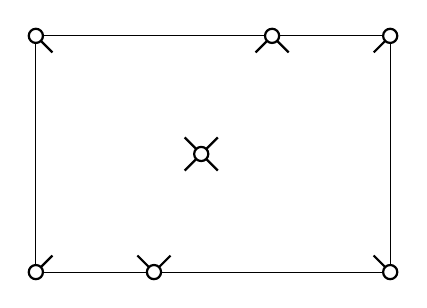
\begin{tikzpicture}[scale=3]
  \coordinate (a) at (0,0);
  \coordinate (b) at (1.5, 0);
  \coordinate (c) at (1.5, 1);
  \coordinate (d) at (0, 1);
  
  \draw (a) rectangle (c);

  \draw[thick] (a) -- (0.07, 0.07);
  \draw[thick, fill=white] (a) circle (0.03);
  
  \draw[thick] (1.5, 1) -- (1.43, 0.93);
  \draw[thick, fill=white] (c) circle (0.03);  

  \draw[thick] (0, 1) -- (0.07, 0.93);
  \draw[thick, fill=white] (0, 1) circle (0.03);  
  
  \draw[thick] (1.5, 0) -- (1.43, 0.07);
  \draw[thick, fill=white] (1.5, 0) circle (0.03);    
  
  \draw[thick] (0.5, 0) -- (0.57, 0.07);
  \draw[thick] (0.5, 0) -- (0.43, 0.07);
  \draw[thick, fill=white] (0.5, 0) circle (0.03);
  
    \draw[thick] (1, 1) -- (0.93, 0.93);
  \draw[thick] (1, 1) -- (1.07, 0.93);
  \draw[thick, fill=white] (1,1) circle (0.03);
  
  \draw[thick] (0.7, 0.5) -- (0.77, 0.57);
  \draw[thick] (0.7, 0.5) -- (0.63, 0.57);
  \draw[thick] (0.7, 0.5) -- (0.77, 0.43);
  \draw[thick] (0.7, 0.5) -- (0.63, 0.43);
  \draw[thick, fill=white] (0.7, 0.5) circle (0.03);
\end{tikzpicture}
\caption{Some decorated points `detected' by $R$}
\label{fig:decoratedpoints}
\end{figure}

When $\V$ is decomposable, $\mu_\V$ is easy to describe.

\begin{proposition}
\label{prop-decomposable-diagram}
Let $V = \bigoplus \I^{l_i}$ be a decomposable persistence module with intervals $\{ l_i \}$. Then
\begin{align*}
\mu_\V(R) = \left | \{ l_i \st l_i \in R \} \right |
\end{align*}
\end{proposition}
\begin{proof}
This follows from the discussion above and Proposition~\ref{quiver-direct-sums}.
\end{proof}

\subsection{Equivalence}

We now have a mechanism to pass from persistence modules to r-measures. In this section we show that every finite r-measure uniquely determines a multiset of decorated points.

\begin{definition}
The \emph{r-interior} of a region $\mathcal{D} \subseteq \R^2$ is the set of decorated points:
\begin{align*}
\mathcal{D}^\rint = \{ (p^*, q^*) \st \text{there exists } R \in \Rect(\mathcal{D}) \text{ with } (p^*, q^*) \in R \}.
\end{align*}
\end{definition}

The r-interior of a region is all the points that are `detected' by an r-measure on that region. For example, the upper half plane $\mathcal{H} = \{ (p, q) \st p \leq q \}$ has r-interior:
\begin{align*}
\mathcal{H}^\rint = \{ (p^*, q^*) \st p < q \} \cup \{ (p^-, p^+) \st p \in \R \}.
\end{align*}

\begin{theorem}[Equivalence]\label{r-measure-equivalence}
Let $\mathcal{D} \subseteq \R^2$. There is a bijection between 
\begin{itemize}
\item r-measures on $\mathcal{D}$ such that $\mu(R) < \infty$ for every $R \in \Rect(\mathcal{D})$; and
\item multisets of decorated points $\mathsf{A}$ in $\mathcal{D}^\rint$ such that $\card(\mathsf{A}|_R) < \infty$ for every $R \in \Rect(\mathcal{D})$,
\end{itemize}
where the measure corresponding to a multiset $\mathsf{A}$ is given by the formula
\begin{align*}
\mu(R) = \card(\mathsf{A}|_R).
\end{align*}
\end{theorem} 

The proof of this theorem occupies the remainder of this section. 

\begin{proof}
One direction of the bijection is easy. Given a multiset $\mathsf{A}$, we define $\mu$ as above. We need only verify that the formula above defines an r-measure. Given any horizontal or vertical split $R = R_1 \cup R_2$, any decorated point $(p^*, q^*) \in R$ belongs to exactly one of $R_1$ and $R_2$. Therefore:
\begin{align*}
\mu(R) = \card(\mathsf{A}|_R) = \card(\mathsf{A}|_{R_1}) + \card(\mathsf{A}|_{R_2}) = \mu(R_1) + \mu(R_2).
\end{align*}

Now for the reverse direction. For an r-measure $\mu$, let $\mathsf{A}$ be the multiset in $\mathcal{D}^\rint$ given by the multiplicity function:
\begin{align*}
m(p^*, q^*) = \min \{ \mu(R) \st R \in \Rect(\mathcal{D}), \, (p^*, q^*) \in R \}.
\end{align*}
This is well defined by the well ordering principle, as each $\mu(R)$ is a non-negative integer.

We must prove that $\mathsf{A}$ satisfies the formula in the statement of the theorem and show that it is the unique such multiset. From above, we know that the multiset $\mathsf{A}$ defines an r-measure $\nu$ via:
\begin{align*}
\nu(R) = \card(\mathsf{A}|_R).
\end{align*}
We now show that $\mu = \nu$ by induction on $\mu(R)$, which is finite by the conditions of the theorem.

In the base case, consider all $R$ such that $\mu(R) = 0$. Let $(p^*, q^*)$ be a point contained in one such $R$. Then:
\begin{align*}
0 \leq m(p^*, q^*) \leq \mu(R) = 0.
\end{align*}
Therefore $m(p^*, q^*) = 0$ inside $R$, and $\nu(R) = \mu(R) = 0$.

Now assume that $\mu(R) = \nu(R)$ for every $R$ with $\mu(R) < k$. We must now show that for any rectangle $R_0$ with $\mu(R_0) = k$, also $\nu(R_0) = k$. Split $R_0$ into four equal quadrants $Q_1, Q_2, Q_3, Q_4$. By finite additivity, we have:
\begin{align*}
\mu(R) &= \mu(Q_1) + \mu(Q_2) + \mu(Q_3) + \mu(Q_4) \\
\nu(R) &= \nu(Q_1) + \nu(Q_2) + \nu(Q_3) + \nu(Q_4).
\end{align*}

If more than one of $\mu(Q_i)$ is non-zero, then $\mu(Q_i) < k$ for all $i$, and the result follows by induction. In the remaining case, there is a single quadrant with measure $k$ and the remainder have measure $0$. Let $R_1$ be this distinguished quadrant.

We now repeat the argument with $R_1$. Either we find the quadrants satisfy $\mu(Q_i) < k$ or there is another quadrant with $\mu(Q_i) = k$. The only unhandled case is when we find an infinite sequence of rectangles $R_0 \supset R_1 \supset \dots$ with $\mu(R_i) = k$ for all $i$. The diameters of the quadrants tend to zero, so the intersection $\bigcap R_i$ contains a single point $(r, s)$.

Therefore, the only contribution to $\nu(R)$ must come from decorated points that belong to all the $R_i$, i.e., decorated points of the form $(r^*, s^*)$. Assume for now that $(r, s)$ lies on the interior of every $R_i$. Divide each $R_i$ into quadrants $R_i^{++}, R_i^{-+}, R_i^{+-}, R_i^{--}$ sharing $(r, s)$ as a common corner, and such that $(r^+, s^+)$ lies in $R_i^{++}$ for all $i$, $(r^-, s^+)$ lies in $R_i^{-+}$, and so on.

The result follows from the following claim: Let $(\varepsilon_i)$ and $(\eta_i)$ be non-increasing sequences of positive real numbers that converge to $0$. Then:
\begin{align*}
m(r^+, s^+) = \lim_{i\to\infty} \mu([r, r+\varepsilon_i] \times [s, s+\eta_i]).
\end{align*}

To see that this is true, let $R$ be a rectangle that contains $(r^+, s^+)$. Then for $i$ sufficiently large, $R_i \subseteq R$. By monotonicity, $\mu(R_i)$ must eventually stabilise to a finite limit. Then:
\begin{align*}
m(r^+, s^+) \leq \min \mu(R_i) = \lim_{i \to \infty} \mu(R_i) \leq \mu(R).
\end{align*}
Now, taking the minimum over all $R$, the RHS becomes $m(r^+, s^+)$ and we have the equality we require.

Returning to the proof of the theorem, we have $m(r^+, s^+) = \lim_{i\to\infty} \mu(R_i^{++})$, with the sequence eventually stabilising at this value. We also have the obvious equivalent statements for the remaining decorated points $(r^*, s^*)$. 

For sufficiently large $i$, we therefore have:
\begin{align*}
\nu(R_0) &= m(r^+, s^+) + m(r^+, s^-) + m(r^-, s^+) + m(r^-, s^-) \\
&= \mu(R_i^{++}) + \mu(R_i^{-+}) + \mu(R_i^{+-}) + \mu(R_i^{--}) = \mu(R_i) = k.
\end{align*}

If $(r, s)$ does not lie in the interior of every $R_i$ then beyond some $N$, the point $(r, s)$ lies on the boundary of $R_i$ for all $i > N$. We then have fewer cases to consider: if $(r, s)$ is on an edge then only two decorated points of the form $(r^*, s^*)$ lie in every $R_i$. If $(r, s)$ is on a corner then only one decorated point needs to be considered. In either case, the above argument goes through.

By induction, we have $\mu(R) = \nu(R)$ for every rectangle $R$. All that remains is to show uniqueness. Let $\mathsf{B}$ be some other multiset with associated r-measure $\nu'$ such that $\mu = \nu'$. We must show that $\mathsf{A} = \mathsf{B}$.

Let $m'(p^*, q^*)$ be the multiplicity function for $\mathsf{B}$, and consider any point $(p^*, q^*) \in \mathcal{D}^\rint$. Let $R$ be a rectangle with $(p^*, q^*)$ at a corner. Because $\nu(R) = \nu'(R) = \mu(R) < \infty$, we can choose a rectangle such that $(p^*, q^*)$ is the only point with positive multiplicity in $R$. Then:
\begin{align*}
m(p^*, q^*) = \nu(R) = \mu(R) = \nu'(R) = m'(p^*, q^*).
\end{align*}
Therefore $m = m'$ for all $(p^*, q^*) \in \mathcal{D}^\rint$ and $\mathsf{A} = \mathsf{B}$.
\end{proof}

The theorem leads to the following definitions.

\begin{definition}
The \emph{decorated diagram} $\Dgm(\V)$ of a persistence module $\V$ is the unique multiset of decorated points such that:
\begin{align*}
\mu_\V(R) = \card(\Dgm(\V)|_R)
\end{align*}

If we forget the topology of the `intervals' we have the \emph{undecorated diagram} $\dgm(\V)$. This is a multiset of ordinary points in $\mathcal{D}$ defined by:
\begin{align*}
\dgm(\V) = \{ (p, q) \st (p^*, q^*) \in \Dgm(\V) \} \cap \text{int } \mathcal{D}
\end{align*}
where `$\text{int } \mathcal{D}$' denotes the ordinary interior of $\mathcal{D}$.
\end{definition}

Proposition~\ref{prop-decomposable-diagram} implies that for any persistence module $\V$ that decomposes into interval modules, $\Dgm(\V)$ is precisely the set of intervals in the decomposition.

\subsection{q-tame persistence modules}

The stability theorem of later sections requires a condition on the structure maps of the persistence modules. This condition is quite natural and is satisfied in practical applications, as demonstrated by the theorems of this section.

\begin{definition}
A persistence module is \emph{q-tame} if for any $s < t$, the structure map $v_s^t$ has finite rank.
\end{definition}

Such modules are called `q-tame' because, for any infinite quadrant $[-\infty, b] \times [c, +\infty]$ we have:
\begin{align*}
\mu_\V([-\infty, b] \times [c, +\infty]) = \langle \qon{b} \qem \qon{c} \st \V \rangle = \rank v_b^c < \infty.
\end{align*}

Note that q-tameness does not mean there are no limit points in the persistence diagram, as we may have limit points on the diagonal $\Delta = \{(x, x) \st x \in \R \}$. By limit point, we mean a point such that every neighbourhood of that point contains infinitely many other points.

\begin{example}
The module
\begin{align*}
\V = \bigoplus_{n=1}^\infty \I[0, \tfrac{1}{n}]
\end{align*}
is q-tame with $\dgm(\V) = \{ (0, \tfrac{1}{n}) \st n \geq 1 \}$. This has an limit point at $(0, 0)$.
\end{example}

We now give some examples of how q-tame modules occur in the wild. Our original motivation for studying persistence modules was to understand persistent homology in the setting of finite simplicial complexes. The results in the remainder of this work apply as a result of the following theorem.

\begin{theorem}
\label{thm-simplicial-qtame}
Let $X$ be the geometric realisation of a finite simplicial complex, and $f : X \to \mathbb{R}$ a continuous function. Then the persistence module $H(X^f)$ induced by the sublevelset filtration of $X$ is q-tame.
\end{theorem}
\begin{proof}
Let $X^a$ denote the sublevel set $X^a = f^{-1}((-\infty, a])$. We must show that, for any $a < b$, $H(X^a) \to H(X^b)$ has finite rank.

Begin with any triangulation of $X$ and repeatedly subdivide the simplices of $X$ until no simplex intersects both $A = f^{-1}(a)$ and $B = f^{-1}(b)$. To see that this is always possible, note that because $X$ is compact and both $A$ and $B$ are closed, $A$ and $B$ are themselves compact. Because $A$ and $B$ are compact subsets of $X$, the function $d(x, B)$ attains a minimum on $A$. This minimum $\varepsilon$ must be nonzero, as $A$ and $B$ are disjoint. We therefore subdivide the simplices until the length of every edge is less than $\varepsilon/2$.

Let $Y$ be the the union of every closed simplex that meets $X^a$. Then $Y$ is a finite simplicial complex, and we have inclusions $X^a \subseteq Y \subseteq X^b$. 

The map $H(X^a) \to H(X^b)$ therefore factorises as $H(X^a) \to H(Y) \to H(X^b)$. Because $Y$ is a finite simplicial complex, $H(Y)$ is finite dimensional and $H(X^a) \to H(X^b)$ has finite rank.
\end{proof}

The Vietoris-Rips complex of a finite set must be a finite simplicial complex, and any simplicial filtration of such a complex leads to a q-tame persistence module. The following theorem shows that a much larger class of metric spaces also lead to a q-tame persistence modules. \cite{chazal2013geometric}

\begin{definition}
A metric space is \emph{totally bounded} if, for any $\varepsilon > 0$, the space can be covered with a finite number of open balls of radius $\varepsilon$.
\end{definition}

Any compact metric space is totally bounded. For any $\varepsilon$, construct the cover with an open ball of radius $\varepsilon$ at every point. By compactness there is a finite subcover which is precisely the cover we require.

\begin{theorem}
\label{thm-tb-qtame}
Let $(X, d_X)$ be a totally bounded metric space. Then the persistence module $H(\mathbf{VR}(X, \alpha))$ is q-tame.
\end{theorem}
\begin{proof}(Outline)
Here we provide a sketch of the proof as the full details are not relevant to the rest of this work. Again we must show that, for any $a < b$, $H(\mathbf{VR}(X, a)) \to H(\mathbf{VR}(X, b))$ has finite rank. Let $\varepsilon = (b-a)/2$. Because $X$ is totally bounded, there is a finite subset $Y \subset X$ such that for any $x \in X$, there is a $y \in Y$ with $d_X(x, y) < \varepsilon / 2$. Let $C$ be some (multivalued) matching between the elements of $X$ and $Y$ so that $d_Y(x, C(x)) \leq \varepsilon / 2$.

Let $\sigma \in \mathbf{VR}(X, a)$, and $\tau \subseteq C(\sigma)$ any finite subset. For any $y, y' \in \tau$ there exist $x, x' \in \sigma$ such that $y \in C(x), y' \in C(x')$ and therefore:
\begin{align*}
d_Y(y, y') \leq d_X(x, x') + \varepsilon \leq a + \varepsilon.
\end{align*}
It follows that $\tau \in \mathbf{VR}(Y, a + \epsilon)$. Symmetrically, for any $\tau \in \mathbf{VR}(Y, a + \epsilon)$, $\sigma' \subseteq C(\tau) \in \mathbf{VR}(X, a + 2 \epsilon)$.

After a little work, this implies the factorisation:
\begin{align*}
H(\mathbf{VR}(X, a)) \to H(\mathbf{VR}(Y, a+\varepsilon)) \to H(\mathbf{VR}(X, a+ 2 \varepsilon)) = H(\mathbf{VR}(X, b)).
\end{align*}
Again, the vector space $H(\mathbf{VR}(Y, a+\varepsilon))$ is finite dimensional so the structure maps all have finite rank.
\end{proof}
\section{Stability}
\label{section-stability}

With the necessary foundations all in place, we can now prove the stability theorem. For the persistence diagram of a data set to be a useful invariant, we would hope that small changes in the data lead to small changes in the persistence diagram. The stability theorem shows that this is the case, once we have pinned down the correct definitions for a `small change' in data and a `small change' in persistence diagram.

\begin{theorem}[Stability]
Let $f, g : X \to \R$ be functions on a topological space $X$ and let $\U = H(X^f), \V = H(X^g)$ be the sublevel persistence modules. If $\U$ and $\V$ are q-tame, then:
\begin{align*}
d_b(\dgm(\U), \dgm(\V)) \leq \Vert f - g \Vert_\infty
\end{align*}
where $d_b$ denotes the `bottleneck distance' between two diagrams, yet to be defined, and $\Vert \cdot \Vert_\infty$ denotes the supremum norm.
\end{theorem}

In this section we will prove the stability theorem after first proving two preliminary results: the box lemma and interpolation lemma.

The stability theorem was first proven in a much more restricted setting by Cohen-Steiner, Edelsbrunner and Harer \cite{cohen2007stability}. They required that $X$ be a triangulable space and that $f$ and $g$ be `tame' functions, i.e., functions with only finitely many homological critical values. Such restrictions are lifted here, following arguments by Chazal et al. \cite{chazal2009proximity} that were later simplified by the same authors \cite{chazal2012structure}.

\subsection{Interleaving distance}

Our first step is to translate the distance $\Vert f - g \Vert_\infty$ into an algebraic statement about persistence modules. Let us suppose $\Vert f - g \Vert_\infty < \delta$. Then for any $x \in X$ we have $f(x) < g(x) + \delta$ and $g(x) < f(x) + \delta$, which implies the following inclusion of sublevel sets:
\begin{align*}
f^{-1}((-\infty, a]) &\subseteq g^{-1}((-\infty, a+\delta]) \subseteq f^{-1}((-\infty, a+2\delta])\\
g^{-1}((-\infty, a]) &\subseteq f^{-1}((-\infty, a+\delta]) \subseteq g^{-1}((-\infty, a+2\delta]).
\end{align*}
These induce maps $U_a \to V_{a+\delta} \to U_{a + 2\delta}$ and $V_a \to U_{a+\delta} \to V_{a + 2\delta}$ for all $a \in \R$. What we have is \emph{almost} an isomorphism of persistence modules, but where the maps in each direction shift the index by $\delta$.

\begin{definition}
A \emph{homomorphism of degree $\delta$} from $\U$ to $\V$ is a collection of maps $\phi_t : U_t \to V_{t+\delta}$ such that:
\begin{displaymath}
\xymatrix{
U_s \ar[d]_{\phi_s} \ar[r]^{u_s^t} & U_t \ar[d]^{\phi_t}\\
V_{s+\delta} \ar[r]^{v_{s+\delta}^{t+\delta}} & V_{t+\delta}
}
\end{displaymath}
commutes for all $s \leq t$. We write $\Hom^\delta(\U, \V)$ for the collection of all such homomorphisms.
\end{definition}

As an example, the ordinary structure maps $v_t^{t+\delta}$ form a homomorphism of degree $\delta$. We write this homomorphism as $1_\V^\delta$.

When we have two mutually `inverse' shift maps as above, we say that $\U$ and $\V$ are $\delta$-interleaved. More precisely:

\begin{definition}
Two persistence modules $\U$ and $\V$ are \emph{$\delta$-interleaved} if there are maps $\Phi \in \Hom^\delta(\U, \V)$ and $\Psi \in \Hom^\delta(\V, \U)$ such that
\begin{align*}
\Psi \Phi = 1_\U^{2\delta}, \quad \Phi \Psi = 1_\V^{2\delta}
\end{align*}
Expanding the maps involved, these equations state that for every $t \in \R$, the following two diagrams commute:
\begin{align*}
\xymatrix@=1em{
U_t \ar[dr] \ar[rr] & & U_{t+2\delta} \\
& V_{t+\delta} \ar[ur]
}
\text{\raisebox{-15pt}{, }}
\quad
\xymatrix@=1em{
& U_{t+\delta} \ar[dr] \\
V_t \ar[ur] \ar[rr] & & V_{t+2\delta}
}
\end{align*}
\end{definition}

Note that a $0$-interleaving is precisely an isomorphism.

If two modules $\U$ and $\V$ are $\delta$-interleaved, they are certainly $(\delta + \epsilon)$-interleaved for any $\epsilon > 0$. We can construct the required maps easily:
\begin{align*}
\Phi' &= \Phi 1_\U^\epsilon \\
\Psi' &= \Psi 1_\V^\epsilon.
\end{align*}
Then
\begin{align*}
\Phi' \Psi' = \Phi 1_\U^\epsilon \Psi 1_\V^\epsilon = 1_\V^\epsilon \Phi \Psi 1_\V^\epsilon = 1_\V^\epsilon 1_\V^{2\delta} 1_\V^\epsilon = 1_\V^{2(\delta + \epsilon)}
\end{align*}
with the $\Psi' \Phi'$ direction identical.

This suggests that we can measure the distance between two persistence modules by finding the smallest $\delta$ for which the modules are $\delta$-interleaved.

\begin{definition}
\label{def-interleaving-distance}
The \emph{interleaving distance} between two persistence modules is:
\begin{align*}
d_i(\U, \V) &= \inf \{ \delta \st \U, \V \text{ are } \delta\text{-interleaved} \}.
\end{align*}
\end{definition}

In the case of sublevel persistence modules, we have the inequality
\begin{align*}
d_i(\U, \V) \leq \Vert f - g \Vert_\infty
\end{align*}
by the discussion above.

The $\inf$ in this definition is not necessarily attained. For example, the two interval modules $\I[p, q)$ and $\I[p, q]$ have interleaving distance 0, but the two modules are clearly not isomorphic.

\begin{proposition}
The interleaving distance satisfies the triangle inequality:
\begin{align*}
d_i(\U, \W) \leq d_i(\U, \V) + d_i(\V, \W)
\end{align*}
for any three persistence modules $\U, \V, \W$.
\end{proposition}
\begin{proof}
Let $(\Phi_1$, $\Psi_1)$ be a $\delta_1$-interleaving between $\U$ and $\V$, and $(\Phi_2$, $\Psi_2)$ a $\delta_2$-interleaving between $\V$ and $\W$. The compositions $\Phi = \Phi_2 \Phi_1$ and $\Psi = \Psi_1 \Psi_2$ yield a $\delta = (\delta_1 + \delta_2)$-interleaving between $\U$ and $\W$. To confirm this is a valid interleaving, we calculate:
\begin{align*}
\Psi \Phi = \Psi_1 \Psi_2 \Phi_2 \Phi_1 = \Psi_1 1_\V^{2\delta_2} \Phi_1 = \Psi_1 \Phi_1 1_\U^{2\delta_2} = 1_\U^{2\delta_1} 1_\U^{2\delta_2} = 1_\U^{2\delta} \\
\Phi \Psi = \Phi_2 \Phi_1 \Psi_1 \Psi_2  = \Phi_2 1_\V^{2\delta_1} \Psi_2 = \Phi_2 \Psi_2 1_\W^{2\delta_1} = 1_\W^{2\delta_2} 1_\W^{2\delta_1} = 1_\W^{2\delta}.
\end{align*} 

Now, taking the infimum over $\delta_1$ and $\delta_2$ we have our result.
\end{proof}

\subsection{Bottleneck distance}

We now define the distance on the other side of the stability theorem, the `bottleneck distance'. The intuition here is that two diagrams are close if we can match the points of the two diagrams such that the distance between paired points is small. There is some subtlety when we have points close to the diagonal $\Delta$. We allow such points to be `matched' to the diagonal so that the appearance of small features does not prevent a matching of the remaining points.

Again we work in the open half plane given by:
\begin{align*}
\mathcal{H} = \{(p, q) \st p < q \}.
\end{align*}

The distance between points is calculated using the $\ell^\infty$-metric. In $\R^2$, this distance is
\begin{align*}
d^\infty((p, q), (r, s)) = \max(|p - r|, |q - s|)
\end{align*}
for two points and
\begin{align*}
d^\infty((p, q), \Delta) = \tfrac{1}{2} (q - p)
\end{align*}
for a point and the diagonal. This use of $\ell^\infty$ is not arbitrary, as the following propositions show.

\begin{proposition}
Let $\U = \I(p^*, q^*)$ and $\U = \I(r^*, s^*)$ be interval modules. Then:
\begin{align*}
d_i(\U, \V) \leq d^\infty((p, q), (r, s))
\end{align*}
\end{proposition}
\begin{proof}
We must show that for any $\delta > d^\infty((p, q), (r, s))$, the modules $\U$ and $\V$ are $\delta$-interleaved. There is an obvious candidate interleaving: set the interleaving maps to $1$ when both the domain and codomain are $\mathbf{k}$ and $0$ otherwise.

First we show that this definition gives us valid module homomorphisms of degree $\delta$. This is equivalent to verifying that the diagram
\begin{displaymath}
\xymatrix{
U_t \ar[d] \ar[r] & U_{t'} \ar[d]\\
V_{t+\delta} \ar[r] & V_{t'+\delta}
}
\end{displaymath}
commutes. Because the spaces and maps are all either $1$ or $0$, the only possible obstruction is some diagram of the form:
\begin{align*}
\xymatrix{
\bullet \ar[d] \ar[r] & \bullet \ar[d]\\
\circ \ar[r] & \bullet
}
\quad
\text{\raisebox{-15pt}{ or }}
\quad
\xymatrix{
\bullet \ar[d] \ar[r] & \circ \ar[d]\\
\bullet \ar[r] & \bullet
}
\end{align*}
In the first case, we must have $p^* < t$ and $t + \delta < r^*$, but $\delta > r-p$ so this is impossible. In the second case, we have $q^* < t'$ and $t' + \delta < s^*$, but $\delta > s-q$. Therefore, $\Phi : \U \to \V$ is a module homomorphism of degree $\delta$. By symmetry, $\Psi : \V \to \U$ is also a valid homomorphism.

Finally, we must show that $\Phi$ and $\Psi$ satisfy $\Psi \Phi = 1_\U^{2\delta}$ and $\Phi \Psi = 1_\V^{2\delta}$. For the first identity, we have the following diagram.
\begin{align*}
\xymatrix@=1em{
U_t \ar[dr] \ar[rr] & & U_{t+2\delta} \\
& V_{t+\delta} \ar[ur]
}
\end{align*}
This can only fail to commute in the following case:
\begin{align*}
\xymatrix{
\bullet \ar[dr] \ar[rr] & & \bullet \\
& \circ \ar[ur]
}
\end{align*}
The top row implies that $p^* < t < t+2\delta < q^*$. Because $\delta > r-p$ and $\delta > q - s$, we have:
\begin{align*}
r^* < (p+\delta)^* < t+\delta < (q-\delta)^* < s^*.
\end{align*}
Therefore $t+\delta$ lies in the interval $(r^*, s^*)$ and the above situation is impossible.

The other identity follows by symmetry. We conclude that $\U$ and $\V$ are interleaved for all $\delta > d^\infty((p, q), (r, s))$, and therefore $d_i(\U, \V) \leq d^\infty((p, q), (r, s))$.
\end{proof}

\begin{proposition}
Let $\U = \I(p^*, q^*)$ be an interval module, and $0$ denote the zero persistence module. Then:
\begin{align*}
d_i(\U, 0) = d^\infty((p, q), \Delta).
\end{align*}
\end{proposition}
\begin{proof}
Because one of the modules is the zero module, all interleaving maps must be the zero map. The only condition that could fail is $\Psi \Phi = 1_\U^{2\delta}$, i.e., $0 = 1_\U^{2\delta}$. This holds when $\delta > \tfrac{1}{2}(q-p)$ and fails when $\delta < \tfrac{1}{2}(q-p)$.
\end{proof}

As we can match points to the diagonal, we weaken our notion of bijection to the following.

\begin{definition}
A \emph{partial matching} between two multisets $\mathsf{A}$ and $\B$ is a subset $\mathsf{M}$ of $\mathsf{A} \times \B$ such that:
\begin{itemize}
\item for every $\alpha \in \mathsf{A}$ there is at most one $\beta \in \B$ such that $(\alpha, \beta) \in \mathsf{M}$; and,
\item for every $\beta \in \B$ there is at most one $\alpha \in \mathsf{A}$ such that $(\alpha, \beta) \in \mathsf{M}$.
\end{itemize}
\end{definition}

\begin{definition}
A partial matching is a \emph{$\delta$-matching} when:
\begin{itemize}
\item for every $(\alpha, \beta) \in \mathsf{M}$, $d^\infty(\alpha, \beta) \leq \delta$;
\item if $\alpha \in \mathsf{A}$ is unmatched then $d^\infty(\alpha, \Delta) \leq \delta$;
\item if $\beta \in \B$ is unmatched then $d^\infty(\beta, \Delta) \leq \delta$.
\end{itemize}
\end{definition}

We now define the bottleneck distance in a similar manner to the interleaving distance.

\begin{definition}
The \emph{bottleneck distance} between two multisets in $\mathcal{H}$ is:
\begin{align*}
d_b(\mathsf{A}, \B) = \inf \{ \delta \st \text{there exists a $\delta$-matching between $\mathsf{A}$ and $\B$}\}.
\end{align*}
\end{definition}

\begin{proposition}
The interleaving distance satisfies the triangle inequality
\begin{align*}
d_b(\A, \mathsf{C}) \leq d_b(\A, \B) + d_b(\B, \mathsf{C})
\end{align*}
for any three multisets $\A, \B, \mathsf{C}$.
\end{proposition}
\begin{proof}
Let $\M_1$ be a $\delta_1$-matching between $\A$ and $\B$, and $\M_2$ a $\delta_2$ matching between $\B$ and $\mathsf{C}$. We define a $\delta = (\delta_1 + \delta_2)$-matching between $\A$ and $\mathsf{C}$ by:
\begin{align*}
\M = \{ (a, \gamma) \st \text{there exists } \beta \in \B \text{ such that } (\alpha, \beta) \in \M_1, (\beta, \gamma) \in \M_2\}.
\end{align*}

If $(\alpha, \gamma) \in \M$, then there is a $\beta$ linking $\alpha$ and $\gamma$, so $d^\infty(\alpha, \gamma) \leq d^\infty(\alpha, \beta) + d^\infty(\beta, \gamma) \leq \delta_1 + \delta_2 = \delta$.

If $\alpha$ is unmatched in $\M$, there are two possibilities. If $\alpha$ is unmatched in $\M_1$ then $d^\infty(\alpha, \Delta) \leq \delta_1 \leq \delta$. If $\alpha$ is matched with $\beta$ in $\M_1$ then $\beta$ must be unmatched in $\M_2$, in which case:
\begin{align*}
d^\infty(\alpha, \Delta) \leq d^\infty(\alpha, \beta) + \delta^\infty(\beta, \Delta) \leq \delta_1 + \delta_2 = \delta.
\end{align*}

The same argument shows that if $\gamma$ is unmatched in $\M$ then $d^\infty(\gamma, \Delta) \leq \delta$. Therefore $\M$ is a valid matching. The proposition follows by taking the infimum over all matchings $\M_1$ and $\M_2$.
\end{proof}

When we work in the realm of q-tame persistence modules, we can show that the $\inf$ is attained. 

\begin{theorem}
\label{thm-bottleneck-inf-attained}
Let $\mathsf{A}$ and $\B$ be locally finite multisets in $\mathcal{H}$. If for every $\eta > \delta$ there exists an $\eta$-matching between $\A$ and $\B$ then there exists a $\delta$-matching.
\end{theorem}
\begin{proof}
Let $\M_n$ be a $(\delta + \tfrac{1}{n})$-matching for all $n \geq 1$. We will construct a $\delta$-matching $\M$ as the `limit' of this sequence. Let $\chi, \chi_n : \A \times \B \to \{0, 1\}$ denote the indicator functions of $\M$ and $\M_n$.

We construct $\chi$ as follows. Because $\A$ and $\B$ are locally finite, they must be countable. Fix an enumeration $(a_\ell, b_\ell)$ of $\A \times \B$. We inductively define a descending sequence:
\begin{align*}
\N = \N_0 \supseteq \N_1 \supseteq \dots \supseteq \N_\ell \supseteq \dots
\end{align*}
such that $\chi_n(a_\ell, b_\ell)$ has the same value for all $n \in \N_\ell$. The descending nature of the sequence means that $\chi_n(a_\ell, b_\ell)$ also agrees for all $\chi_n$ in $\N_{\ell'}$ with $\ell' > \ell$. We can then define $\chi(a_\ell, b_\ell)$ to be this common value.

Given $\N_{\ell-1}$, consider the two sets
\begin{align*}
\{n \in \N_{\ell-1} \st \chi_n(a_\ell, b_\ell) = 0\} \text{ and } \{n \in \N_{\ell-1} \st \chi_n(a_\ell, b_\ell) = 1\}.
\end{align*}
At least one of these sets infinite, and we define $\N_\ell$ to be one such infinite set. This construction guarantees that we never run out of `choices' for the next set of $\chi_n$.

We now must prove that this $\chi$ is a valid $\delta$-matching between $\A$ and $\B$. First, note that for any finite subset $F \in \A \times \B$, there exists an $\chi_N$ beyond which $\chi$ agrees with $\chi_n$ on $F$ for all $n \geq N$. Indeed, choose $N$ to be the largest index $\ell$ of all pairs in $F$. By the definition of $\chi$, the claim holds.

We can now check the conditions for a $\delta$-matching.
\begin{itemize}
\item For $a \in \A$, there is at most one $b \in \B$ with $\chi(a, b) = 1$.
\begin{proof}
Suppose $a$ is matched with both $b$ and $b'$. By the claim above, there must be an $n$ such that $\chi_n(a, b) = \chi_n(a, b') = 1$, which contradicts the fact that $\chi_n$ is a valid partial matching.
\end{proof}
\item For $b \in \B$, there is at most one $a \in \A$ with $\chi(a, b) = 1$.
\begin{proof}
Follows symmetrically.
\end{proof}
\item For $a \in \A$, if $d^\infty(a, \Delta) > \delta$, there is a $b \in \B$ with $\chi(a, b) = 1$.
\begin{proof}
Choose $N$ such that $d^\infty(a, \Delta) > \delta + \tfrac{1}{N}$. The set:
\begin{align*}
F = \{b \in \B \st d^\infty(a, b) \leq \delta + \tfrac{1}{N} \}
\end{align*}
is finite, as $\B$ is locally finite and this set lies away from the diagonal. By the claim above, there an $\ell$ for which $\chi(a, b) = \chi_n(a, b)$ for all $b \in F$ and $n \in \N_\ell$. Also, if $n \geq N$ then $\chi_n(a, b) = 1$ for some $b \in F$, as $\M_n$ is a $(\delta + \tfrac{1}{n})$-matching. Therefore $\chi(a, b) = \chi_n(a, b) = 1$ for some $b \in \B$.
\end{proof}
\item For $b \in \B$, if $d^\infty(b, \Delta) > \delta$, there is a $a \in \A$ with $\chi(a, b) = 1$.
\begin{proof}
Follows symmetrically.
\end{proof}
\item If $\chi(a, b) = 1$, then $d^\infty(a, b) \leq \delta$.
\begin{proof}
There exist infinitely many $n \in \N$ such that $\chi_n(a, b) = 1$. For all such $n$, the equation $d^\infty(a, b) \leq \delta + \tfrac{1}{n}$ holds. Because $n$ becomes arbitrarily large, the result follows.
\end{proof}
\end{itemize}

This completes the proof of the theorem.
\end{proof}

\subsection{Interpolation lemma}

The first main ingredient of the stability theorem is the interpolation lemma, which proves that for any interleaved pair of persistence modules, there is a 1-parameter family of modules that interpolates between them. We begin by giving an alternative characterisation of an interleaving between two modules.

The plane $\R^2$ has a partial order on it defined by 
\begin{align*}
(p_1, q_1) \leq (p_2, q_2) \text{ whenever } p_1 \leq p_2 \text{ and } q_1 \leq q_2
\end{align*}
For any real number $x$, we define shifted diagonal $\Delta_x$ to be:
\begin{align*}
\Delta_x = \{ (p, q) \st q-p=2x \} \subset \R^2.
\end{align*}
Any persistence modules over $\R$ can be then considered as a persistence module over $\Delta_x$, by identifying each $t \in \R$ with the point $(t-x, t+x) \in \Delta_x$. 

\begin{proposition}
Two persistence modules $\U$, $\V$ are $|y-x|$-interleaved if and only if there is a persistence module $\W$ over $\Delta_x \cup \Delta_y$ such that $\W_{\Delta_x} = \U$ and $\W_{\Delta_y} = \V$.
\end{proposition}
\begin{proof}
Let $\delta = |y-x|$, and let us assume $x < y$. In addition to the maps within each of $\Delta_x$ and $\Delta_y$, we also have maps between the two lines. Let $\Phi = \{\phi_t\}$ be the vertical maps from $\Delta_x$ to $\Delta_y$ and $\Psi = \{\psi_t\}$ the horizontal maps from $\Delta_y$ to $\Delta_x$. Then $\phi_t$ and $\psi_t$ are maps:
\begin{align*}
\phi_t : U_t = W_{t-x, t+x} &\to W_{t-x, t+2y-x} = V_{t+\delta}\\
\psi_t : V_t = W_{t-y, t+y} &\to W_{t+y-2x, t+y} = U_{t+\delta}.
\end{align*}
The composition law for $\W$ implies that $\Psi\Phi=1_\U^{2\delta}$ and $\Phi\Psi=1_\V^{2\delta}$ as required.

The module $\W$ does not contain more information than the interleaving, as any map $w_S^T$ can be factored into the form:
\begin{align*}
w_S^T &= u_s^t &&\text{ if } S, T \in \Delta_x \\
w_S^T &= v_s^t &&\text{ if } S, T \in \Delta_y \\
w_S^T &= v_{s+\delta}^t \phi_s &&\text{ if } S \in \Delta_x \text{ and } T \in \Delta_y \\
w_S^T &= u_{s+\delta}^t \psi_s &&\text{ if } S \in \Delta_y \text{ and } T \in \Delta_x.
\end{align*}
\end{proof}

\begin{lemma}[Interpolation lemma]
Let $\U$ and $\V$ be $\delta$-interleaved modules. Then there exists a family of persistence modules $\{\U_x \st x \in [0, \delta]\}$ such that $\U_0 = \U$, $\U_\delta = \V$ and $\U_x$, $\U_y$ are $|y-x|$ interleaved for all $x, y \in [0, \delta]$.
\end{lemma}
\begin{proof}
In view of the previous proposition, this is equivalent to showing that there exists a persistence module $\overline\W$ over the strip $\Delta_{[0, \delta]}$ where $\overline\W|_{\Delta_0} = \U$ and $\overline\W|_{\Delta_\delta} = \V$. Then, any restriction to $\Delta_x \cup \Delta_y$ provides the required interleavings for $x,y \in [0, \delta]$.

To simplify the proof, we begin by scaling and translating the plane so that the interval $[0, \delta]$ is replaced with $[-1, 1]$. The $\delta$-interleaving between $\U$ and $\V$ gives us a persistence module $\W$ over $\Delta_{-1} \cup \Delta_1$.

We wish to construct two persistence modules over the strip $\Delta_{[-1, 1]}$ and a map $\Omega$ between them. The persistence module $\overline\W$ will be the image of this map.

We first construct four persistence modules over all of $\mathbf{R}^2$ as follows.
\begin{align*}
\mathbb{A} &= \U[p-1] &\text{ given by } A_{(p, q)} &= U_{p-1} &\text{ and } a_{(p, q)}^{(r, s)} &= u_{p-1}^{r-1} \\
\mathbb{B} &= \V[q-1] &\text{ given by } B_{(p, q)} &= V_{q-1} &\text{ and } b_{(p, q)}^{(r, s)} &= v_{q-1}^{s-1} \\
\mathbb{C} &= \U[q+1] &\text{ given by } C_{(p, q)} &= U_{p+1} &\text{ and } c_{(p, q)}^{(r, s)} &= u_{q+1}^{s+1} \\
\mathbb{D} &= \V[p+1] &\text{ given by } D_{(p, q)} &= V_{q+1} &\text{ and } d_{(p, q)}^{(r, s)} &= v_{p+1}^{r+1}
\end{align*}

We now define four module maps by abuse of notation:
\begin{align*}
1_\U : \mathbb{A} &\to \mathbb{C} &\text{ defined at } &(p, q) \text{ to be } &u_{p-1}^{q+1} : U_{p-1} &\to U_{q+1}\\
\Phi : \mathbb{A} &\to \mathbb{D} &\text{ defined at } &(p, q) \text{ to be } 
&\phi_{p-1} : U_{p-1} &\to V_{p+1}\\
\Psi : \mathbb{B} &\to \mathbb{C} &\text{ defined at } &(p, q) \text{ to be } &\psi_{q-1} : V_{q-1} &\to U_{q+1}\\
1_\V : \mathbb{B} &\to \mathbb{D} &\text{ defined at } &(p, q) \text{ to be } &v_{q-1}^{p+1} : V_{q-1} &\to V_{p+1}.
\end{align*}

The maps $\Phi$ and $\Psi$ are the interleaving maps and are defined on all of $\mathbf{R}^2$. The map $1_\U$ is defined whenever $p-1 \leq q+1$, and $1_\V$ is defined when $q-1 \leq p+1$. It follows that all four are maps are defined when $-2 \leq q - p \leq 2$. This is precisely the region $\Delta_{[-1, 1]}$.

Now let $\Omega \in \Hom(\mathbb{A} \oplus \mathbb{B}, \mathbb{C} \oplus \mathbb{D})$ be the map given by the following matrix:
\begin{align*}
\Omega = \begin{pmatrix}
1_\U & \Psi \\
\Phi & 1_\V
\end{pmatrix}.
\end{align*}

We claim that $\overline\W = \im(\Omega)$ is the persistence module over $\Delta_{[-1, 1]}$ that we require. The only thing to verify is that $\U \cong \overline\W|_{\Delta_{-1}}$ and $\V \cong \overline\W|_{\Delta_1}$.

On $\Delta_{-1} = \{(t+1, t-1)\}$ we have:
\begin{align*}
(\mathbb{A} \oplus \mathbb{B})_t &= U_t \oplus V_{t-2} \\
(\mathbb{C} \oplus \mathbb{D})_t &= U_t \oplus V_{t+2}
\end{align*}
and
\begin{align*}
\omega_t = \begin{pmatrix}
u_t^t & \psi_{t-2} \\
\phi_t & v_{t-2}^{t+2}
\end{pmatrix}.
\end{align*}

Note that the map $v_{t-2}^{t+2}$ can be factorized using the interleaving maps as $\phi_t \psi_{t-2}$. We then have:
\begin{align*}
\omega_t = \begin{pmatrix}
1 & \psi_{t-2} \\
\phi_t & v_{t-2}^{t+2}
\end{pmatrix}
= \begin{pmatrix}
1 & \psi_{t-2} \\
\phi_t & \phi_t \psi_{t-2}
\end{pmatrix}
= \begin{pmatrix}
1 \\ \phi_t
\end{pmatrix} 
\begin{pmatrix}
1 & \psi_{t-2}
\end{pmatrix},
\end{align*}
which, when written as a diagram of modules, takse the form
\begin{align*}
\U \oplus \V[t-2] \overset{\Omega_1}{\longrightarrow} \U \overset{\Omega_2}{\longrightarrow} \U \oplus \V[t+2],
\end{align*}
where
\begin{align*}
\Omega_1(U_t \oplus V_t) = U_t + \Psi(V_t) \quad \text{ and } \quad \Omega_2(U_t) = U_t \oplus \Phi(U_t).
\end{align*}

Note that $\Omega_1$ is surjective and $\Omega_2$ is injective for every $t$. Therefore $\U \cong \im(\Omega|_{\Delta_{-1}})$.

The argument for $\V \cong \overline\W|_{\Delta_1}$ is almost identical. On $\Delta_{-1} = \{(t-1, t+1)\}$ the modules are
\begin{align*}
(\mathbb{A} \oplus \mathbb{B})_t &= U_{t-2} \oplus V_t \\
(\mathbb{C} \oplus \mathbb{D})_t &= U_{t+2} \oplus V_t
\end{align*}
and $\Omega$ is
\begin{align*}
\omega_t = \begin{pmatrix}
u_{t-2}^{t+2} & \psi_t \\
\phi_{t-2} & v_t^t
\end{pmatrix}
= \begin{pmatrix}
\psi_t \phi_{t-2} & \psi_t \\
\phi_{t-2} & 1
\end{pmatrix}
= \begin{pmatrix}
\psi_t \\ 1
\end{pmatrix} 
\begin{pmatrix}
\phi_{t-2} & 1
\end{pmatrix}
\end{align*}

This is equivalent to 
\begin{align*}
\U[t-2] \oplus \V \overset{\Omega_3}{\longrightarrow} \V \overset{\Omega_4}{\longrightarrow} \U[t+2] \oplus \V
\end{align*}
where
\begin{align*}
\Omega_3(U_t \oplus V_t) = \Phi(U_t) + V_t \quad \text{ and } \quad \Omega_4(V_t) = \Phi(V_t) \oplus V_t
\end{align*}

Again we have $\Omega_3$ surjective and $\Omega_4$ injective, so $\V \cong \im(\Omega|_{\Delta_{1}})$.
\end{proof}

\subsection{Box lemma}

The second ingredient of the stability theorem is the box lemma, which allows us to relate the persistence diagrams of two interleaved persistence modules locally.

Let $R = [a, b] \times [c, d]$ be a rectangle in $\R^2$. The \emph{$\delta$-thickening} of $R$, written $R^\delta$, is the rectangle:
\begin{align*}
  R^\delta = [a - \delta, b + \delta] \times [c - \delta, d + \delta].
\end{align*}

We will also refer to the thickening of a single point. If $\alpha = (p, q)$, then:
\begin{align*}
  \alpha^\delta = [p - \delta, p + \delta] \times [q - \delta, q + \delta].
\end{align*}

\begin{lemma}[Box lemma]
Let $\U$, $\V$ be $\delta$-interleaved persistence modules. Let $R$ be a rectangle. Then $\mu_\U(R) \leq \mu_\V(R^\delta)$ and $\mu_\V(R) \leq \mu_\U(R^\delta)$.
\end{lemma}
\begin{proof}
Let $R = [a, b] \times [c, d]$ and $R^\delta = [A, B] \times [C, D]$. We have the following persistence modules:
\begin{align*}
  \U_{a,b,c,d} : U_a \to U_b \to U_c \to U_d
\end{align*}
and
\begin{align*}
  \U_{A,B,C,D} : V_A \to V_B \to V_C \to V_D
\end{align*}
by restricting to the appropriate finite sets. The interleaving maps allow us to combine these persistence modules:
\begin{align*}
  \W : V_A \overset{\Psi_A}{\longrightarrow} U_a \longrightarrow U_b \overset{\Phi_b}{\longrightarrow} V_B \longrightarrow V_C \overset{\Psi_C}{\longrightarrow} U_c \longrightarrow U_d \overset{\Phi_d}{\longrightarrow} V_D
\end{align*}
where $\Phi : \U \to \V$ and $\Psi : \V \to \U$ are the interleaving maps. We now calculate:
\begin{align*}
\mu_\V(R^\delta) &= \langle \Qoff{A} \qem \qno \qem \qno \qem \Qon{B} \qem \Qon{C} \qem \qno \qem \qno \qem \Qoff{D} \st \V \rangle \\
&= \langle \Qoff{A} \qem \qno \qem \qno \qem \Qon{B} \qem \Qon{C} \qem \qno \qem \qno \qem \Qoff{D} \st \W \rangle \\
&= \langle \Qoff{A} \qem \qoff{a} \qem \qon{b} \qem \Qon{B} \qem \Qon{C} \qem \qon{c} \qem \qoff{d} \qem \Qoff{D} \st \W \rangle + \text{other terms}\\
&\geq \langle \Qoff{A} \qem \qoff{a} \qem \qon{b} \qem \Qon{B} \qem \Qon{C} \qem \qon{c} \qem \qoff{d} \qem \Qoff{D} \st \W \rangle \\
&= \langle \Qno \qem \qoff{a} \qem \qon{b} \qem \Qno \qem \Qno \qem \qon{c} \qem \qoff{d} \qem \Qno \st \W \rangle \\
&= \langle \Qno \qem \qoff{a} \qem \qon{b} \qem \Qno \qem \Qno \qem \qon{c} \qem \qoff{d} \qem \Qno \st \U \rangle \\
&= \mu_\U(R).
\end{align*}

The other inequality follows by symmetry.
\end{proof}

\subsection{The stability theorem}

Finally, we combine the above results to prove the stability theorem. Recall the statement:

\begin{theorem}[Stability]
Let $f, g : X \to \R$ be functions on a topological space $X$ and let $\U = H(X^f), \V = H(X^g)$ be the sublevel persistence modules. If $\U$ and $\V$ are q-tame, then:
\begin{align*}
d_b(\dgm(\U), \dgm(\V)) \leq \Vert f - g \Vert_\infty.
\end{align*}
\end{theorem}

The first step is to apply the inequality $d_i(\U, \V) \leq \Vert f - g \Vert_\infty$. The stability theorem can be proven by showing that:
\begin{align*}
d_b(\dgm(\U), \dgm(\V)) \leq d_i(\U, \V).
\end{align*}
In other words,

\begin{proposition}
\label{prop-stability-1}
Let $\U$, $\V$ be q-tame persistence modules that are $\eta$-interleaved for all $\eta > \delta$. Then there exists a $\delta$-matching between $\dgm(\U)$ and $\dgm(\V)$.
\end{proposition}

In view of Theorem~\ref{thm-bottleneck-inf-attained}, this is a consequence of the following easier proposition:

\begin{proposition}
Let $\U$, $\V$ be q-tame persistence modules that are $\delta$-interleaved. Then there exists a $\delta$-matching between $\dgm(\U)$ and $\dgm(\V)$.
\end{proposition}

Proposition~\ref{prop-stability-1} follows, because if there is a $\eta$-matching for all $\eta > \delta$, then there is a $\delta$-matching.

The interpolation lemma states that there exists a family of persistence modules $\{\U_x \mid x \in [0, \delta]\}$ such that $\U_x$ and $\U_y$ are $|y-x|$-interleaved for all $x, y \in [0, \delta]$. Let $\{\mu_x\}$ be the associated r-measures.

First we show that the `Hausdorff distance' between $\dgm(\mu_x)$ and $\dgm(\mu_y)$ is always less than $|y-x|$. Intuitively, the Hausdorff distance is similar to the bottleneck distance but we are permitted to match multiple points from one diagram to a single point in the other. 

\begin{lemma}
Let $\A = \dgm(\mu_x)$, $\B = \dgm(\mu_y)$ and $\eta = |y-x|$. Then:
\begin{itemize}
\item If $a \in \A$ and $d^\infty(a, \Delta) > \eta$ then there exists $b \in \B$ with $d^\infty(a, b) \leq \eta$; and,
\item If $b \in B$ and $d^\infty(b, \Delta) > \eta$ then there exists $a \in \A$ with $d^\infty(a, b) \leq \eta$.
\end{itemize}
\end{lemma}
\begin{proof}
Let $a \in A$ be a point such that $d^\infty(a, \Delta) > \eta$. Choose an $\varepsilon$ such that $\eta + \varepsilon < d^\infty(a, \Delta)$. 

By the box inequality, 
\begin{align*}
1 \leq \mu_x(a^\varepsilon) \leq \mu_y(a^{\eta + \varepsilon})
\end{align*}
and we have at least one point of $\B$ in $a^{\eta + \varepsilon}$. Because $\varepsilon$ was arbitrary and $\B$ is locally finite, there must be at least one point $b$ of $\B$ in $a^\eta$. It follows that $d^\infty(a, b) \leq \eta$.

The second statement follows symmetrically.
\end{proof}

We now prove the theorem when $\dgm(\mu_x)$ is finite for all $x$. Once we have done this, we can finish off the proof of the main theorem using a compactness argument. For convenience we will write $\A_x = \dgm(\mu_x)$.

\begin{lemma}
If $\A_x$ is finite for all $x$, then the theorem holds.
\end{lemma}
\begin{proof}
We claim that for every $x \in [0, \delta]$, there exists a number $\rho(x) > 0$ such that $\A_x, \A_y$ are $|y-x|$-matched whenever $|y - x| < \rho(x)$.

Let $a_1, \dots, a_k$ be the distinct points of $\A_x$, with $n_1, \dots, n_k$ their multiplicities. Define $\rho(x)$ to be:
\begin{align*}
\rho(x) = \min \begin{cases}
\tfrac{1}{2} d^\infty(a_i, \Delta) & \text{ for all } i\\
\tfrac{1}{2} d^\infty(a_i, a_j) & \text{ for all } i, j.
\end{cases}
\end{align*}

We must show that if $|y-x| < \rho(x)$ then $\A_x, \A_y$ are $|y-x|$-matched. Let $\eta = |y-x|$. By $\Delta^\eta$, we mean the thickening:
\begin{align*}
\Delta^\eta &= \{\alpha \in \R^2 \st d^\infty(\alpha, \Delta) \leq \eta\} \\
&= \{(p, q) \in \R^2 \st q - p \leq 2 \eta\}.
\end{align*}

By the previous lemma, $\A_x$ and $\A_y$ have Hausdorff distance less than $\eta$. It follows that $\A_y$ is contained in the closed set:
\begin{align*}
\Delta^\eta \cup \alpha_1^\eta \cup \dots \cup \alpha_k^\eta.
\end{align*}
The definition of $\rho(x)$ is chosen so that all of these sets are disjoint.

Choose $\epsilon > 0$ so that $2\eta + \varepsilon < 2 \rho(x)$. For every box $a_i^\eta$, the box lemma implies:
\begin{align*}
n_i = \mu_x(a_i^\varepsilon) \leq \mu_y(a_i^{\eta+\varepsilon}) \leq \mu_x(a_i^{2\eta+\varepsilon}) = n_i.
\end{align*}
We can therefore match the $n_i$ copies of $a_i$ with the points of $\A_y$ that are in the square $a_i^\eta$, for all $i$. The only unmatched points are the ones in $\Delta^\eta$, so this defines a valid partial matching.

This shows that $\A_0$ and $\A_\delta = \B$ are $\delta$-matched by the following argument.

The triangle inequality for matchings states that if $\A_0$, $\A_x$ are $x$-matched, and $\A_x$, $\A_y$ are $|y-x|$-matched, then $\A_0$, $\A_y$ are $y$-matched. We must show that we can continue matching in this way until $\A_0$ and $\A_\delta$ are $\delta$-matched.

Let $m = \sup \{x\in [0, \delta] \st \text{$A_0$ and $A_x$ are $x$-matched}\}$. First we show that this $\sup$ is attained. Choose an $m'$, such that $m - m' < \rho(m)$. Then $\A_0$ and $\A_{m'}$ are $m'$-matched by the definition of $m$, and $\A_{m'}$ and $\A_m$ are $|m'-m|$-matched by the argument above. Therefore $\A_0$ and $\A_m$ are $m$-matched.

Finally, we must have $m = \delta$. If $m < \delta$ then there exists a $m''$ with $m < m'' < \delta$ and $m'' - m < \rho(m)$. Again we have that $\A_0$ and $\A_{m''}$ are $m''$-matched, contradicting the definition of $m$.

Therefore $\A_0$ and $\A_\delta$ are $\delta$-matched.
\end{proof}

\begin{theorem}
The stability theorem holds, without assuming each $\A_x$ is finite.
\end{theorem}
\begin{proof}
We prove this using a similar compactness argument to Theorem~\ref{thm-bottleneck-inf-attained}. Let $\{\H_n\}$ be an increasing sequence of open subsets of $\H$ such that the union of these sets is $\H$ and each $\H_n$ has compact closure.

Because each $\A_x$ is locally finite, we have that $\A_x \cap \H_n$ is finite for all $x$ and $n$. By the previous lemma, for each $n$ we have a $\delta$-matching $\M_n$ between $\A_0 \cap \H_n$ and $\A_\delta \cap \H_n$.

We now reuse the construction and arguments of Theorem~\ref{thm-bottleneck-inf-attained} to get a limit multiset $\M$. We must now verify that this $M$ gives a $\delta$-matching. Firstly, every matched pair is separated by at most $\delta$, as this is true for every $\M_n$. Secondly, every $a \in \A_0$ is matched with at most one $b \in \A_\delta$ and vice versa, for the same reason as before.

All that remains to be checked is that every $a \in \A_0$ with $d^\infty(a, \Delta) > \delta$ is matched. Consider the thickening $a^\delta$ for some such $a$. This square is compact and contained in $\H$, so must be contained in $\H_n$ for $n$ sufficiently large. Therefore $a$ is matched in $\M_n$ for $n$ sufficiently large. Because $\A_\delta$ is locally finite, $\alpha$ has only finitely many points within $\delta$ distance from $a$. As in the earlier theorem, there exists an $n$ beyond which the matchings $\M_n$ all agree on this finite set. Because the $\M_n$ are all valid matchings, we conclude that $a$ is matched with some $b$ in $\M$.

By symmetry, any $b \in \A_\delta$ with $d^\infty(b, \Delta) > \delta$ is matched in $\M$, so $\M$ is the required matching.
\end{proof}

\section{Category Theory Primer}
\label{section-category-theory}

Like much of algebraic topology, the theory of persistence modules has been reinterpreted using the language of category theory. This section introduces the main concepts used in category theory and shows how many of the constructions we've seen fit into this viewpoint.

In the following chapter we will use these techniques to prove a strong structure theorem for q-tame persistence modules.

\begin{definition}
A \emph{category} $\C$ consists of:
\begin{itemize}
\item a class $\Ob(\C)$ of objects;
\item for every $a, b \in \Ob(\C)$, a class $\Hom(a, b)$ of morphisms; and,
\item for every $a, b, c \in \Ob(\C)$, a binary operation
\begin{align*}
\Hom(b, c) \times \Hom(a, b) &\to \Hom(a, c), \qquad (g, f) \mapsto g\circ f \text{ or } gf
\end{align*}
\end{itemize}
such that:
\begin{itemize}
\item morphism composition is \emph{associative}: if $f : a \to b$, $g : b \to c$ and $h : c \to d$ then $f \circ (g \circ h) = (f \circ g)\circ h$; and,
\item every object has an \emph{identity} morphism: for every $a \in \Ob(\C)$, there exists a morphism $1_a \in \Hom(a, a)$ such that for every $f : x \to a$, $1_a \circ f = f$ and for every $g : a \to y$, $g \circ 1_a = g$.
\end{itemize}
\end{definition}

Many familiar mathematical objects form a category. We have the categories:
\begin{itemize}
\item $\mathbf{Set}$, of sets and functions;
\item $\mathbf{Top}$, of topological spaces and continuous maps;
\item $\mathbf{Grp}$, of groups and homomorphisms; and,
\item $\mathbf{Vect}_\mathbf{k}$, of $\mathbf{k}$-vector spaces and linear maps.
\end{itemize} 
It is routine to check that these classes satisfy the conditions for a category above.

The morphisms in a category are often functions with some added conditions, but this is not always the case. Given any poset $P$, we can consider $P$ as a category by taking the elements of $P$ as our objects, and including precisely one morphism $s \to t$ for each $s \leq t$.

We can apply category theory to the study of persistence because, given a indexing poset $P$, the class of persistence modules together with module homomorphisms forms a category $\mathbf{Pers}_P$. 

A \emph{subcategory} $\mathcal{S}$ of a category $\C$ is a category with objects and morphisms subcollections of the objects and morphisms of $\C$. We require that these objects and morphisms form a valid category.

A subcategory $\mathcal{S}$ is \emph{full} if for every $a, b \in \Ob(\mathcal{S})$, we have $\Hom_\mathcal{S}(a, b) = \Hom_\C(a, b)$. In other words, $\mathcal{S}$ includes all the morphisms between $a$ and $b$ that exist in $\C$.

\subsection{Functors and natural transformations}

The next fundamental concept in category theory is the notion of a \emph{functor} between two categories.

\begin{definition}
Given two categories $\C, \D$, a \emph{functor} $F : \C \to \D$ is a mapping that assigns:
\begin{itemize}
\item to every object $c \in \C$ an object $F(c) \in \D$; and,
\item to every morphism $f : x \to y$ in $\C$, a morphism $F(f) : F(x) \to F(y)$ in $\D$
\end{itemize}
such that:
\begin{align*}
F(1_a) &= 1_{F(a)} \\
F(g \circ f) &= F(g) \circ F(f).
\end{align*}
\end{definition}

The most important example of a functor we have seen so far is homology. If the ground ring is a field $\k$, then $H_n(-) : \mathbf{Top} \to \mathbf{Vect}_\k$ is a functor assigning to each space $X$ the $n$-dimensional homology of $X$, and to each continuous map $f : X \to Y$ the linear map given by Theorem~\ref{homology-functor}.

In fact, persistence modules themselves can be thought of as functors. Let $P$ be a poset. Then persistence modules over $P$ are precisely functors $\V : P \to \mathbf{Vect}_\k$, where we consider $P$ as a category using the construction earlier.

Moving up the abstraction tower, we can also define \emph{natural transformation}s between two functors.

\begin{definition}
Given two functors $F, G : \C \to \D$, a \emph{natural transformation} $\tau : F \natto G$ is a function that assigns to every object $c \in \C$, a morphism $\tau_c : F(c) \to G(c)$ in $\D$, such that for every $f : c \to c'$ in $\C$, the diagram
\begin{displaymath}
\xymatrix{
F(c) \ar[d]_{F(f)} \ar[r]^{\tau_c} & G(c) \ar[d]^{G(f)}\\
F(c') \ar[r]^{\tau_{c'}} & G(c')
}
\end{displaymath}
commutes.
\end{definition}

If we choose two categories $\C, \D$, we can form the \emph{functor category} $[\C, \D]$ which has as its objects the class of all functors $\C \to \D$, and morphisms the natural transformations between them.
 
A module homomorphism $\U \to \V$ is precisely a natural transformation between the modules, when we consider the modules as functors. We can therefore make the identification $\mathbf{Pers}_P = [P, \mathbf{Vect}_\k]$.

\subsection{Limits and colimits}

The utility of category theory becomes apparent when we consider the `universal' objects that often appear in mathematics. A common template for new constructions is to find the simplest object that satisfies certain properties. 

Consider the `direct product' operation on sets. In the case of sets, we know the direct product $A \times B$ is the collection of all ordered pairs $(a, b)$ with $a \in A, b \in B$. We could instead characterise the direct product as the `universal' object with maps to the two components.

\begin{definition}
The direct product of two sets $A$ and $B$ is the unique set $A \times B$ with two maps $\pi_1 : A \times B \to A$ and $\pi_2 : A \times B \to B$ such that whenever some other set $C$ exists with maps $\phi_1 : C \to A$, $\phi_2 : C \to B$, these maps factor through a unique map $u : C \to A \times B$.
\begin{displaymath}
\xymatrix{
& C \ar@/_1pc/[ddl]_{\phi_1} \ar@/^1pc/[ddr]^{\phi_2} \ar@{-->}[d]_u & \\
& A \times B \ar[dl]_{\pi_1} \ar[dr]^{\pi_2} & \\
A & & B
}
\end{displaymath}
\end{definition}

A \emph{limit} in category theory is the generalisation of this idea.

\begin{definition}
Let $F : \mathcal{J} \to \C$ be a functor. A \emph{cone to $F$} is an object $C$ of $\C$ together with a family of morphisms $\phi_X : C \to F(X)$ for every $X \in \mathcal{J}$, such that the following diagram commutes for every $f : X \to Y$ in $\mathcal{J}$.
\begin{displaymath}
\xymatrix{
& C \ar[dl]_{\phi_X} \ar[dr]^{\phi_Y}  & \\
F(X) \ar[rr]_{F(f)} & & F(Y)
}
\end{displaymath}

The \emph{limit} of $F$ is a cone $(L, \pi_X)$ to $F$ such that for any other cone $(C, \phi_X)$ to $F$, there is a unique morphism $u : C \to L$ such that $\phi_X = \pi_X \circ u$ for all $X \in \mathcal{J}$. In other words, there exists a morphism $u$ making the following diagram commute:
\begin{displaymath}
\xymatrix{
& C \ar@/_1pc/[ddl]_{\phi_X} \ar@/^1pc/[ddr]^{\phi_Y} \ar@{-->}[d]_u & \\
& L \ar[dl]_{\pi_X} \ar[dr]^{\pi_Y} & \\
F(X) \ar[rr]_{F(f)} &  & F(Y)
}
\end{displaymath}

A limit is \emph{small} if in the indexing category $\mathcal{J}$, the collection of objects and morphisms forms a set and not a proper class.
\end{definition}

We recover the above example when we set $\mathcal{J}$ to the discrete category $\{1, 2\}$, $\C$ to the category $\mathbf{Set}$, and $F$ to the functor assigning $F(1) = A$ and $F(2) = B$.

A \emph{colimit} is the categorical dual of a limit, which we can define by reversing the arrows in the definition above.

\begin{definition}
Let $F : \mathcal{J} \to \C$ be a functor. A \emph{cocone from $F$} is an object $C$ of $\C$ together with a family of morphisms $\phi_X : F(X) \to C$ for every $X \in \mathcal{J}$, such that the following diagram commutes for every $f : X \to Y$ in $\mathcal{J}$.
\begin{displaymath}
\xymatrix{
F(X) \ar[rr]^{F(f)} \ar[dr]_{\phi_X} & & F(Y) \ar[dl]^{\phi_Y} \\
& C &
}
\end{displaymath}

The \emph{colimit} of $F$ is a cocone $(L, \pi_X)$ from $F$ such that for any other cocone $(C, \phi_X)$ from $F$, there is a unique morphism $u : L \to C$ such that $\phi_X = u \circ \pi_X$ for all $X \in \mathcal{J}$. In other words, there exists a morphism $u$ making the following diagram commute:
\begin{displaymath}
\xymatrix{
F(X) \ar[rr]^{F(f)} \ar[dr]_{\pi_X} \ar@/_1pc/[ddr]_{\phi_X} & & F(Y) \ar[dl]^{\pi_Y} \ar@/^1pc/[ddl]^{\phi_Y} \\
& L \ar@{-->}[d]_u & \\
& C &
}
\end{displaymath}
\end{definition}

If we choose $\mathcal{J} = \{1, 2\}$, $\C = \mathbf{Set}$, and $F$ the functor $F(1) = A$ and $F(2) = B$ as before, the colimit of $F$ is the disjoint union $A \coprod B$. The maps $\pi_1, \pi_2$ are then the inclusions of $A$ and $B$ into $A \coprod B$.

Limits and colimits do not necessarily always exist. A category is called \emph{complete} if it contains all small limits, and \emph{cocomplete} if it contains all small colimits. The categories $\mathbf{Set}$ and $\mathbf{Vect}_\mathbf{k}$ are both complete and cocomplete.
\newcommand{\Pers}{\mathbf{Pers}}
\renewcommand{\Ob}{\mathbf{Ob}}
\newcommand{\Eph}{\mathbf{Eph}}

\section{The Observable Category}
\label{section-observable}

We have seen throughout the previous sections of this work that persistence modules over $\R$ are quite badly behaved. Not every persistence module decomposes into interval modules. We restrict our attention to q-tame persistence modules, but even those do not always decompose into interval modules.

We then defined the persistence diagram as an invariant for q-tame persistence modules, but it is not a complete invariant: two non-isomorphic q-tame persistence modules can have the same persistence diagram.

In a recent paper, Chazal et al. \cite{chazal2014observable} show that these deficiencies vanish completely if we make a small adjustment to the category we are working in. Philosophically, the important data carried by persistence modules is how information persists over intervals, so features that exist over short intervals are seen as unimportant. Taken to the extreme we have what we refer to as \emph{ephemeral features}; features that exist only over a single point.

In this section we will construct the \emph{observable category} of persistence modules $\Ob$, where such ephemeral information is ignored by design. We then show that this category has all the properties we could want: every q-tame module decomposes into a sum of interval modules and the persistence diagram is a complete invariant.

We again restrict our attention to persistence modules over $\R$. To simplify the notation, we will write $\Pers$ to mean $\mathbf{Pers}_\R$.

\subsection{Construction}

First, a more formal definition of the persistence modules we are eliminating.

\begin{definition}
An \emph{ephemeral module} is one where the structure maps $v_s^t$ are 0 for all $s < t$.
\end{definition}

The collection of all ephemeral modules and morphisms forms a category $\mathbf{Eph}$, which is a full subcategory of $\Pers$. We now define a weaker notion of isomorphism, where two modules are considered equivalent if they only differ by ephemeral modules.

\begin{definition}
A \emph{weak isomorphism} is a module homomorphism $\Phi$ such that both $\ker \Phi$ and $\coker \Phi$ are ephemeral modules. Recall that, for persistence modules, kernels and cokernels are done pointwise.
\end{definition}

For example, consider the module map $\Phi : \I[p, q] \to \I[p, q)$, given by $\phi_t = 1$ where both domain and codomain are $\k$. Then $\Phi$ is a weak isomorphism as $\ker \Phi = \I[q,q] $ and $\coker \Phi = 0$, both ephemeral.

We now wish to construct the `quotient category' $\Pers / \Eph$, which we refer to as the \emph{observable category} $\mathbf{Ob}$. By quotient category, we mean that we have a quotient functor $\pi : \Pers \to \Ob$ satisfying the following universal property: $\pi$ sends all weak isomorphisms of $\Pers$ to actual isomorphisms in $\Ob$, and any other functor $
F : \Pers \to \mathcal{C}$ that also sends weak isomorphisms to isomorphisms factors uniquely through $\pi$.

In problems of this sort there is often no explicit construction of the quotient category. In this case, however the objects and morphisms of $\Ob$ are easy to describe. We will give the construction of $\Ob$ first and then verify that it satisfies the universal property.

Ordinary module morphisms in $\Pers$ are collections of linear maps $\phi_t : U_t \to V_t$. In what follows, it will be more useful to think of them as maps $\phi_s^t : U_s \to V_t$, such that $\phi_s^t = v_q^t \phi_p^q u_s^p$ whenever $s \leq p \leq q \leq t$. We can convert readily between the two representations by setting $\phi_t = \phi_t^t$ in one direction, and $\phi_s^t = \phi_t u_s^t = v_s^t \phi_s$ in the other. With this in mind:

\begin{definition}
An \emph{observable morphism} or \emph{ob-morphism}, $\Phi^\circ : \U \dashrightarrow \V$, is a collection of linear maps $\phi_s^t : U_s \to V_t$ for all $s < t$, such that $\phi_s^t = v_q^t \phi_p^q u_s^p$ whenever $s \leq p < q \leq t$. Note that, in contrast with ordinary morphisms, $s$ must be strictly less than $t$.

If $\Phi^\circ : \U \dashrightarrow \V$ and $\Psi^\circ : \V \dashrightarrow \W$ are ob-morphisms, the composition $\Psi^\circ \Phi^\circ$ is given by $(\Psi^\circ \Phi^\circ)_s^t = \psi_u^t \phi_s^u$ for any $s < u < t$. The condition above guarantees that this is well defined.
\end{definition}

\begin{definition}
The \emph{observable category} $\Ob$ is the collection of persistence modules together with ob-morphisms. The quotient functor $\pi : \Pers \to \Ob$ maps every object to itself, and every morphism $\Phi = \{ \phi_s^t \st s \leq t \}$ to $\pi(\Phi) = \Phi^\circ = \{ \phi_s^t \st s < t \}$ by forgetting each $\phi_t^t$.
\end{definition}

In the remainder of this section we show that $\Ob$ satisfies the universal property. Theorem \ref{thm-weak-to-iso} shows that $\pi$ sends weak isomorphisms to isomorphisms, and Theorem \ref{thm-universal-property} shows that other functors of this sort must factor uniquely through $\pi$.

\begin{theorem}
\label{thm-weak-to-iso}
If $\Phi : \V \to \W$ is a weak isomorphism then $\Phi^\circ = \pi(\Phi)$ is invertible in $\Ob$ and is therefore an isomorphism.
\end{theorem}
\begin{proof}
We construct an inverse $\Psi^\circ = \{\psi_s^t\}$ as follows. For a given $s < t$, choose an intermediate $s < u < t$. 

Because $\coker \Phi$ is ephemeral, the composition of $w_s^u : W_s \to W_u$ with the natural map $W_u \to \coker \phi_u$ is zero. Otherwise, we would have some subspace of $h \subset V_s$ such that $w_s^u \phi_s(h) = \phi_u v_s^u(h) \subset \coker \phi_u$, which is a contradiction. Therefore, $w_s^u$ factors as a map $\omega_s^u : W_s \to \im \phi_u$ followed by the inclusion of $\im \phi_u$ into $W_u$.

Also, $\ker \Phi$ is ephemeral, so the composition of the inclusion $\ker \phi_u \to V_u$ and $v_u^t : V_u \to V_t$ is zero. We now get an induced map $\tau_u^t : \im \phi_u \to V_t$, so that the composition of this map with the natural map $V_u \to \im \phi_u$ is $v_u^t$.

We now define our inverse map to be $\psi_s^t = \tau_u^t \omega_s^u$. This gives a valid inverse for $\phi$, as each map only `forgets' information in the kernel or cokernel, both of which are ephemeral.
\end{proof}

Given an arbitrary persistence module $\V$, we now construct a `simpler' persistence module $\overline\V$ that captures the non-ephemeral information in $\V$.

\begin{definition}
Let $\V$ be a persistence module. We define $\overline\V$ to be the persistence module with spaces
\begin{align*}
\overline V_t = \colim \: \{V_s \st s < t\}
\end{align*}
and structure maps given by the universal property of colimits. These colimits exist as $\mathbf{Vect}_\mathbf{k}$ is cocomplete.
\end{definition}

This definition is a little opaque, so we unpack it as follows. The collection $\{V_s \st s < t\}$ forms a diagram indexed by all real numbers less than $t$ which we informally represent as follows:
\begin{displaymath}
\xymatrix{
\dots \ar[r] & V_{s_1} \ar[r] & \dots \ar[r] & V_{s_2} \ar[r] & \dots < V_t
}
\end{displaymath}
$\overline V_t$ is then the colimit of this diagram, i.e. the vector space and maps so that
\begin{displaymath}
\xymatrix{
\dots \ar[r] & V_{s_1} \ar[r] \ar@{-}[drrr] & \dots \ar[r] \ar@{-}[drr] & V_{s_2} \ar[r] \ar@{-}[dr] & \dots \ar@{-}[d] & < V_t \\
& & & & \overline V_t
}
\end{displaymath}
is the initial such vector space that makes the diagram commute. If we choose some $u$ with $t < u$, then there is a collection of maps $\{V_{t_i} \to \overline V_u \st t_i < u \}$. In particular, this includes maps from $\{V_{s_i} \to \overline V_u \st s_i < t \}$! Our diagram looks like the following:
\begin{displaymath}
\xymatrix{
% DRR DRR
\dots \ar[r] & V_{s_1} \ar[r] \ar@{-}[drrr] \ar@{-}[drrrrrrr] & \dots \ar[r] \ar@{-}[drr] \ar@{-}[drrrrrr] & V_{s_2} \ar[r] \ar@{-}[dr] \ar@{-}[drrrrr] & \dots \ar[r] \ar@{-}[d] \ar@{-}[drrrr]  & V_{t_1} \ar[r] & \dots \ar[r]  & V_{t_2} \ar[r]  & \dots  \\
& & & & \overline V_t \ar@{-->}[rrrr]_{\overline v_t^u} & & & & \overline V_u
}
\end{displaymath}
By the universal property these maps $\{ V_{s_i} \to \overline V_u \}$ must factor uniquely through $\overline V_t$, and we define the structure map $\overline v_t^u$ to be this map.

\begin{example}
If $\V$ is any interval with endpoints $(p, q)$, then $\overline \V = \I(p, q]$. Looking at $\overline V_p$, this is the colimit of the diagram of maps $\{V_s \st s < p\}$, all of which are 0. The space $\overline V_q$ is the colimit of $\{V_s \st s < q\}$, which are constant $\mathbf{k}$ approaching $q$.
\end{example}

For any ob-morphism $\phi^\circ : \V \dashrightarrow \W$, we can generate maps $\overline V_t \to \overline W_t$ as suggested by the following diagram:
\begin{displaymath}
\xymatrix{
\dots \ar[r] \ar[dr] & V_{s_1} \ar[r] \ar[dr] & \dots \ar[r] \ar[dr] & V_{s_2} \ar[r] \ar[dr] & \dots & < V_t \\
\dots \ar[r] & W_{s_1} \ar[r] \ar@{-}[drrr] & \dots \ar[r] \ar@{-}[drr] & W_{s_2} \ar[r] \ar@{-}[dr] & \dots \ar@{-}[d]& < W_t \\
& & & & \overline W_t
}
\end{displaymath}
By the universal property, the vertical paths to $\overline W_t$ must factor uniquely through a map $\overline V_t \to \overline W_t$, which is the map we require. We can therefore think of `bar' as a functor $\Ob \to \Pers$.

The universal property also generates, for each $t$, a map $\overline V_t \to V_t$. It is straightforward but tedious to verify that this is a module homomorphism $n^\V : \overline \V \to \V$.

\begin{proposition}
Given any persistence module $\V$, the morphism $n^\V : \overline \V \to \V$ is a weak isomorphism.
\end{proposition}
\begin{proof}
As $n^\V$ is a module morphism, for any $s < t$ we have a commutative diagram
\begin{displaymath}
\xymatrix{
\overline V_s \ar[d]_{n^\V_s} \ar[r]^{\overline v_s^t} & \overline V_t \ar[d]^{n^\V_t}\\
V_s \ar[r]_{v_s^t} \ar[ur] & V_t
}
\end{displaymath}
where the diagonal map is given by the universal property of $\overline V_t$. The bottom triangle commutes by the definition of $n^\V$ and the top triangle commutes by the definition of $\overline v_s^t$.

Therefore, the map $\overline v_s^t$ sends $\ker(n^\V_t)$ to zero, which means $\ker(n^\V)$ is ephemeral. Similarly, $v_s^t$ sends $V_s$ to $\im(n^\V_t)$, so therefore to zero in $\coker(n^\V_t)$, and $\coker(n^\V)$ is ephemeral.
\end{proof}

With the groundwork in place, we can now prove the universal property of $\pi$.

\begin{theorem}
\label{thm-universal-property}
Let $F : \Pers \to \C$ be a functor that takes weak isomorphisms to actual isomorphisms. Then there is a unique functor $G : \Ob \to \C$ such that $F = G \pi$.
\end{theorem}
\begin{proof}
Because $\Ob$ has the same objects as $\Pers$, the functor $G$ is uniquely determined on objects. We now consider morphisms.

First consider the diagram:
\begin{displaymath}
\xymatrix{
\overline \V \ar[r]^{\overline \Phi} \ar[d]_{n^\V} & \overline \W  \ar[d]^{n^\W}\\
\V \ar[r]_{\Phi} & \W
}
\end{displaymath}
We wish to show that this diagram commutes. This is equivalent to showing that the diagram of vector spaces
\begin{displaymath}
\xymatrix{
\overline V_t \ar[r]^{\overline \phi_t} \ar[d]_{n^\V_t} & \overline W_t  \ar[d]^{n^\W_t}\\
V_t \ar[r]_{\phi_t} & W_t
}
\end{displaymath}
commutes for all $t$. Consider any space $V_s$ with $s < t$. As $\Phi$ is a module map, we have that the following compositions of maps are equal:
\begin{align*}
V_s \xrightarrow{\phi_s} W_s \xrightarrow{w_s^t} W_t = V_s \xrightarrow{v_s^t} V_t \xrightarrow{\phi_t} W_t
\end{align*}
Now by the universal property of colimits, the maps $v_s^t$ and $w_s^t$ factor through $\overline V_t$ and $\overline W_t$ respectively:
\begin{align*}
V_s \xrightarrow{\phi_s} W_s \to \overline W_t \xrightarrow{n^\W_t} W_t = V_s \to \overline V_t \xrightarrow{n^\V_t} V_t \xrightarrow{\phi_t} W_t
\end{align*}
Now, by the definition of $\overline \Phi$, we can rewrite the left hand side to:
\begin{align*}
V_s \to \overline V_t \xrightarrow{\overline \phi_t} \overline W_t \xrightarrow{n^\W_t} W_t = V_s \to \overline V_t \xrightarrow{n^\V_t} V_t \xrightarrow{\phi_t} W_t
\end{align*}
This holds for \emph{every} $s < t$, so by the uniqueness of the map $\overline V_t \to W_t$, we must have that $n^\W_t \overline \phi_t = \phi_t n^\V_t$ as required.

Now consider an ob-morphism $\Phi^\circ : \V \dashrightarrow \W$. We have a commutative diagram in $\Ob$:
\begin{displaymath}
\xymatrix{
\overline \V \ar@{-->}[r]^{\pi(\overline \Phi)} \ar@{-->}[d]_{\pi(n^\V)} & \overline \W  \ar@{-->}[d]^{\pi(n^\W)}\\
\V \ar@{-->}[r]_{\Phi^\circ} & \W
}
\end{displaymath}
Recall that both $n^\V$ and $n^\W$ are weak isomorphisms, so $\pi(n^\V)$ and $\pi(n^\W)$ are both isomorphisms. If there is a functor $G$ with $F = G \pi$, applying $G$ to the diagram above forces us to define
\begin{align*}
G(\Phi^\circ) = F(n^\W)F(\overline \Phi)F(n^\V)^{-1}
\end{align*}
for every ob-morphism $\Phi^\circ$. This is a valid functor, as if $\Psi^\circ : \W \dashrightarrow \U$ then:
\begin{align*}
G(\Psi^\circ \Phi^\circ) &= F(n^\U)F(\overline{\Psi^\circ \Phi^\circ})F(n^\V)^{-1} \\
&= F(n^\U)F(\overline{\Psi^\circ} \; \overline{\Phi^\circ})F(n^\V)^{-1} \\
&= F(n^\U)F(\overline{\Psi^\circ})F(\overline{\Phi^\circ})F(n^\V)^{-1} \\
&= F(n^\U)F(\overline{\Psi^\circ})F(n^\W)^{-1} F(n^\W) F(\overline{\Phi^\circ})F(n^\V)^{-1} \\
&= G(\Psi^\circ) G(\Phi^\circ).
\end{align*}

Now suppose $\Phi^\circ = \pi(\Phi)$. Returning to the first diagram we considered, we have that:
\begin{displaymath}
\xymatrix{
\overline \V \ar[r]^{\overline \Phi} \ar[d]_{n^\V} & \overline \W  \ar[d]^{n^\W}\\
\V \ar[r]_{\Phi} & \W
}
\end{displaymath}
commutes. Applying $F$,
\begin{align*}
F(\Phi)F(n^\V) &= F(n^\W)F(\overline \Phi),
\intertext{or in other words,}
F(\Phi) &= F(n^\W)F(\overline \Phi)F(n^\V)^{-1}\\
 &= G(\Phi^\circ) = G(\pi(\Phi)).
\end{align*}
Therefore $F = G\pi$ on morphisms and $\pi$ satisfies the universal property.
\end{proof}

The above construction is an example of \emph{localisation}. There is a well developed theory for quotient categories $\C/\mathcal{A}$ when the category $\C$ is an \emph{abelian category}, and $\mathcal{A}$ is a full subcategory satisfying some technical conditions. Here we give a quick overview of the concepts involved.

An abelian category is one that shares many useful properties with $\mathbf{Ab}$, the category of abelian groups. In particular, in an abelian category every morphism has a kernel and cokernel, and each pair of objects has a product and coproduct. If $\C$ is a small category and $\D$ is an abelian category, any functor category $[\C, \D]$ is also abelian, with the relevant operations all performed pointwise.

Because $\mathbf{Vect}_\k$ is abelian, $\Pers = [\R, \mathbf{Vect}_\k]$ is also abelian. This retroactively justifies the algebraic manipulations involving kernels and cokernels that have appeared throughout previous sections of this work.

The theory of localisation shows that when these conditions are satisfied, not only does the quotient $\C/\mathcal{A}$ always exist, but it is also itself an abelian category. Therefore, we do not lose any algebraic power when working in $\Ob$.

A full treatment of localisation can be found in Popescu \cite{popescu1973abelian}.

\subsection{Structure and stability in $\Ob$}

We begin by quoting some decomposition results for persistence modules over $\R$, as given by Crawley-Boevey \cite{chazal2014observable,crawley2012decomposition}. 

\begin{definition}
A sequence \emph{stabilises} if beyond some point the terms in the sequence are all equal. Let $\V$ be a persistence module over $\R$.
\begin{enumerate}[i)]
\item $\V$ has the \emph{descending chain condition on images} if for all $t \geq s_1 > s_2 > \dots$, the chain
\begin{align*}
V_t \supseteq \im(v_{s_1}^t) \supseteq \im(v_{s_2}^t) \supseteq \dots
\end{align*}
stabilises.
\item Given $s \leq t$, the space $V_s$ has the \emph{descending chain condition on $t$-bounded kernels} if for all $t < \dots < r_2 < r_1$ the chain
\begin{align*}
V_s \supseteq \ker(v_s^{r_1}) \supseteq \ker(v_s^{r_2}) \supseteq \dots
\end{align*}
stabilises.
\item $\V$ has the \emph{descending chain condition on sufficient bounded kernels} if for all $t$ and nonzero $v \in V_t$, there exists $s \leq t$ such that $v \in \im(v_s^t)$ and $V_s$ has the descending chain condition on $t$-bounded kernels.
\end{enumerate}
\end{definition}

Note that any q-tame persistence module must have the descending chain condition on images. For all $s < t$, $\rank v_s^t$ is always finite, so $\im(v_s^t)$ must be finite dimensional. The well ordering principle implies that the chain must then stabilise. For a similar reason, in a q-tame persistence module, $V_s$ has the descending chain condition on $t$-bounded kernels for every $s < t$.

However, q-tame persistence modules need not satisfy the descending chain condition on sufficient bounded kernels. Consider the module 
\begin{align*}
\V = \bigoplus_{n=1}^\infty \I[0, \tfrac{1}{n}]
\end{align*}
seen earlier. Because the spaces with $t < 0$ are all $0$, any nonzero $v \in V_0$ is not in the image of any $v_s^0$ with $s < 0$. In the definition we are therefore forced to take $s = 0$. But $V_0$ does not satisfy the descending chain condition on $0$-bounded kernels. To see this, take $r_n = \tfrac{1}{n}$, then:
\begin{align*}
V_0 \supseteq \ker(v_0^1) \supseteq \ker(v_0^{\frac{1}{2}}) \supseteq \ker(v_0^{\frac{1}{3}}) \supseteq \dots
\end{align*}
does not stabilise.

When the conditions do hold, we can use the following theorem.

\begin{theorem}[Crawley-Boevey \cite{crawley2012decomposition}]
Any persistence module with the descending chain condition on images and on sufficient bounded kernels is a direct sum of interval modules.
\end{theorem}

The strategy now is to show that every q-tame persistence module is weakly isomorphic to one that satisfies the above conditions. When we pass through to $\Ob$, this becomes a true isomorphism.

\begin{definition}
The \emph{radical} of a persistence module $\V$ is the submodule $\rad \V$ defined by:
\begin{align*}
(\rad \V)_t = \sum_{s < t} \im(v_s^t).
\end{align*}
\end{definition}

By construction, $\rad \V$ satisfies the descending chain condition on sufficient bounded kernels, as we have eliminated the $v \in V_t$ such that $v \notin \im(v_s^t)$ for any $s < t$. Therefore $\rad \V$ satisfies the conditions of the above theorem and decomposes as a direct sum of interval modules.

\begin{proposition}
The natural inclusion $I = (i_t) : \rad \V \to \V$ is a weak isomoprhism.
\end{proposition}
\begin{proof}
Firstly, $\ker I = 0$ as $I$ is an inclusion, so $\ker I$ is ephemeral. Let $v \notin \im(v_s^t)$ for any $s < t$, so that $v + \im(i_t) \in \coker(i_t)$. For any $u > t$, $v_t^u(v) \in \im(i_t)$ so $v$ is mapped to $0$ in $\coker(i_u)$. We conclude that $\coker I$ is also ephemeral. 
\end{proof}

Therefore, when we pass to $\Ob$ we have the following structure theorem. 

\begin{theorem}
Any q-tame persistence module is isomorphic in $\Ob$ to a direct sum of interval modules.
\end{theorem}

We can transplant the stability result of early sections into $\Ob$, in view of the following propositions.

\begin{proposition}
The interleaving distance between $\U$ and $\V$ is invariant under ob-isomorphisms.
\end{proposition}
\begin{proof}
Suppose $\U$ and $\U'$ are ob-isomorphic. Then $d_i(\U, \U') = 0$, as we can take the ob-isomorphism maps $\{\phi_t^{t+\varepsilon}\}$ as an interleaving for all $\varepsilon > 0$. From the triangle inequality it follows that $d_i(\U, \V) = d_i(\U', \V)$.
\end{proof}

\begin{proposition}
The undecorated persistence diagram is invariant under ob-isomorphisms.
\end{proposition}
\begin{proof}
Let $\Phi : \V \dashrightarrow \W$ be an ob-isomorphism with inverse $\Psi : \W \dashrightarrow \V$. Recall that the undecorated diagram is given by the multiplicity function
\begin{align*}
m(p, q) = \min \{ \mu(R) \st R \in \Rect(\mathcal{D}), \, (p, q) \in R \}.
\end{align*}
We show that $m_\V(p, q) = m_\W(p, q)$ for all $(p, q)$. Let $R = [a, b] \times [c, d]$ be the rectangle that attains the minimum in the definition of $m_\V(p, q)$ and select a rectangle $R' = [a', b'] \times [c', d']$ lying inside $R$ so $(p, q) \in R' \subset R$. Following the same argument as the box lemma, we have:
\begin{align*}
\mu_\V(R) &= \langle \Qoff{A} \qem \qno \qem \qno \qem \Qon{B} \qem \Qon{C} \qem \qno \qem \qno \qem \Qoff{D} \st \V \rangle \\
&\geq \langle \Qoff{A} \qem \qoff{a} \qem \qon{b} \qem \Qon{B} \qem \Qon{C} \qem \qon{c} \qem \qoff{d} \qem \Qoff{D} \st \W \rangle \\
&= \langle \Qno \qem \qoff{a} \qem \qon{b} \qem \Qno \qem \Qno \qem \qon{c} \qem \qoff{d} \qem \Qno \st \U \rangle \\
&= \mu_\U(R')
\end{align*}
and therefore $m_\W(p, q) \leq m_\V(p, q)$. The reverse inequality follows by symmetry, so the two multisets must be equal.
\end{proof}

Therefore, the stability theorem remains true in $\Ob$. 

\begin{proposition}
Let $\V$ and $\W$ be q-tame persistence modules. Then $\V$ and $\W$ are ob-isomorphic if and only if their undecorated persistence diagrams are equal.
\end{proposition}
\begin{proof}
We saw the forwards direction above. For the reverse direction, we know that $\V$ and $\W$ are be ob-isomorphic to direct sums of interval modules. We can choose the intervals to be open and nonempty. These intervals are determined by the persistence diagrams of $\V$ and $\W$. These diagrams are equal, so the two direct sum decompositions are isomorphic. 
\end{proof}

The above proposition shows we have finally come full circle. Just as there is a bijection in standard persistent homology between persistence modules and barcodes, there is a bijection between isomorphism classes of q-tame persistence modules in $\Ob$ and locally finite persistence diagrams.

\newpage
\nocite{*}
\printbibliography

\appendix

\section{Implementation in Haskell}
\label{code-appendix}

The following Haskell code implements the algorithm given by Zomorodian and Carlsson \cite{zomorodian2005computing} for computing the persistence homology of a filtration of a simplicial complex.

\lstset{ %
  basicstyle=\footnotesize,        % the size of the fonts that are used for the code
  breakatwhitespace=true,         % sets if automatic breaks should only happen at whitespace
  breaklines=true,                 % sets automatic line breaking
}

\lstinputlisting[language=Haskell, caption=Algebra.hs]{tophat/Algebra.hs}
\lstinputlisting[language=Haskell, caption=Rational.hs]{tophat/Rational.hs}
\lstinputlisting[language=Haskell, caption=Z2.hs]{tophat/Z2.hs}
\lstinputlisting[language=Haskell, caption=Simplex.hs]{tophat/Simplex.hs}
\lstinputlisting[language=Haskell, caption=Chain.hs]{tophat/Chain.hs}
\lstinputlisting[language=Haskell, caption=Barcode.hs]{tophat/Barcode.hs}
\lstinputlisting[language=Haskell, caption=PersistentHomology.hs]{tophat/PersistentHomology.hs}
\lstinputlisting[language=Haskell, caption=Main.hs]{tophat/Main.hs}


\end{document}
